\documentclass[inputs/ppgc,inputs/diss,english]{iiufrgs}

\usepackage[utf8]{inputenc}
\usepackage{graphicx}
\usepackage{times}
\usepackage[alf,abnt-emphasize=bf]{inputs/abntex2cite}

\usepackage{amsmath}
\usepackage{amssymb}
\usepackage{amsthm}
\usepackage[linesnumbered,ruled,boxed,commentsnumbered]{algorithm2e}
\usepackage[capitalize]{cleveref}
\usepackage{booktabs}
\usepackage{enumitem}
\usepackage{listings}
\usepackage{tikz}
\usepackage[textsize=tiny,colorinlistoftodos,prependcaption]{todonotes}

\usetikzlibrary{arrows.meta}

\input{inputs/formais.def} % this does not work in class options idk why
\newcommand{\mr}[2][noinline]{\todo[#1,fancyline,color=blue!20]{#2}}
\newcommand{\mri}[2][inline]{\todo[#1,fancyline,color=blue!20]{#2}}
\newcommand{\agp}[2][noinline]{\todo[color=orange!60,linecolor={orange!100},#1,fancyline,author=André]{#2}}
\newcommand{\agpi}[2][inline]{\todo[color=orange!60,linecolor={orange!100},#1,fancyline,author=André]{#2}}
\newcommand{\rv}[2][noinline]{\todo[color=red!50,linecolor={red!100},#1,fancyline,author=Rafael]{#2}}
\newcommand{\rvi}[2][inline]{\todo[color=red!50,linecolor={red!100},#1,fancyline,author=Rafael]{#2}}

\providecommand{\floor}[1]{\ensuremath{\left\lfloor #1\right\rfloor}}
\providecommand{\ceil}[1]{\ensuremath{\left\lceil #1\right\rceil}}

\providecommand{\multiset}[1]{\ensuremath{\{\!\!\{#1\}\!\!\}}}
\providecommand{\sas}{\ensuremath{\text{SAS}^{+}}\xspace}
\providecommand{\strips}{STRIPS\xspace}
\providecommand{\astar}{\ensuremath{\text{A}^{*}}\xspace}
\providecommand{\gbfs}{\ensuremath{\text{GBFS}}\xspace}
\providecommand{\wida}{\ensuremath{\text{W-IDA}^{*}}\xspace}
\providecommand{\ida}{\ensuremath{\text{IDA}^{*}}\xspace}
\providecommand{\h}{\ensuremath{h}\xspace}
\providecommand{\hvalue}[1]{\ensuremath{h^{#1}}\xspace}
\providecommand{\hff}{\hvalue{\text{FF}}}
\providecommand{\hgc}{\hvalue{\text{GC}}}
\providecommand{\hstar}{\hvalue{*}}
\providecommand{\hlmc}{\hvalue{\text{lm-c}}}
\providecommand{\hmax}{\hvalue{\text{max}}}
\providecommand{\hadd}{\hvalue{\text{add}}}
\providecommand{\hnn}{$\hat h$\xspace}
\providecommand{\hnrsl}{$\hat h^{\text{N-RSL}}$\xspace}
\providecommand{\hboot}{$\hat h^{\text{Boot}}$\xspace}
\providecommand{\hgc}{\hvalue{\text{gc}}}
\providecommand{\hhgn}{\hvalue{\text{HGN}}}
\providecommand{\unit}{/1\xspace}
\providecommand{\hvfc}{\text{SUI}\xspace}
\providecommand{\hmin}{\text{SAI}\xspace}
\providecommand{\rw}{{RW}\xspace}
\providecommand{\bfs}{{BFS}\xspace}
\providecommand{\dfs}{{DFS}\xspace}
\providecommand{\bfsrw}{\text{FSM}\xspace}
\providecommand{\nn}{{NN}\xspace}
\providecommand{\fssp}{{FSS}\xspace}
\providecommand{\bssp}{{BSS}\xspace}
\providecommand{\hnnrs}{$\hat h{^{20\%}_\text{\meanfx}}$\xspace}
\providecommand{\hnnrsfifty}{$\hat h{^{50\%}_\text{\meanfx}}$\xspace}
\providecommand{\hffexp}{$h^{FF}_{exp}$}
\providecommand{\hgcexp}{$h^{GC}_{exp}$}
\providecommand{\hnnbase}{$\hat h_{0}$\xspace}
\providecommand{\hnnbfs}{$\hat h_{\text{bfs}}$\xspace}
\providecommand{\hnndfs}{$\hat h_{\text{dfs}}$\xspace}
\providecommand{\hnnrw}{$\hat h_{\text{rw}}$\xspace}
\providecommand{\hnnbfsrw}{$\hat h_\text{fsm}$\xspace}
\providecommand{\hnnbfsrwl}[1]{\ensuremath{\hat h_{#1}}\xspace}
\providecommand{\hnnnomutex}{\ensuremath{\hat h^{'}}\xspace}
\providecommand{\hnnnomutexl}[1]{\ensuremath{\hat h^{'}_{#1}}\xspace}
\providecommand{\hnnrsp}[1]{\ensuremath{\hat h_\text{fsm}/^{#1\%}_{\text{RS}}}\xspace}
\providecommand{\hnnrslp}[2]{\ensuremath{\hat h_\text{fsm}^{#1}/^{#2\%}_{\text{RS}}}\xspace}
\providecommand{\define}[1]{#1}
\providecommand{\facts}{\ensuremath{L_F}\xspace}
\providecommand{\meanfx}{\ensuremath{L_{\overline{F}}}\xspace}
\providecommand{\default}{\ensuremath{L_{200}}\xspace}
\providecommand{\distfarthest}{\ensuremath{d^*}\xspace}

%% mathematical definitions
\ifcsname dom\endcsname\else\DeclareMathOperator{\dom}{dom}\fi
\DeclareMathOperator{\pre}{pre}
\DeclareMathOperator{\eff}{eff}
\DeclareMathOperator{\sucs}{succ}
\DeclareMathOperator{\pred}{pred}
\DeclareMathOperator{\functioninitial}{initial\_state}
\DeclareMathOperator{\functiongoal}{goal\_condition}
\DeclareMathOperator{\mutex}{mutex}
\DeclareMathOperator{\del}{del}
\DeclareMathOperator{\add}{add}
\ifcsname R\endcsname\else\newcommand{\R}{\ensuremath{\mathbb{R}}}\fi

\newtheorem{property}{Property}[section]

%% blocks world example
\providecommand{\facton}[2]{\ensuremath{\text{on}(#1,#2)}\xspace}
\providecommand{\factontable}[1]{\ensuremath{\text{on-table}(#1)}\xspace}
\providecommand{\factclear}[1]{\ensuremath{\text{clear}(#1)}\xspace}
\newcommand{\drawCube}[5]{
    \draw[#4!90, fill=#4!50] (#1,#2,#3+#5) -- ++(0,#5,0) -- ++(#5,0,0) -- ++(0,-#5,0) -- cycle; % front
    \draw[#4!90, fill=#4!50] (#1,#2+#5,#3) -- ++(0,0,#5) -- ++(#5,0,0) -- ++(0,0,-#5) -- cycle; % top
    \draw[#4!90, fill=#4!50] (#1+#5,#2,#3) -- ++(0,#5,0) -- ++(0,0,#5) -- ++(0,-#5,0) -- cycle; % right
}


\title{Understanding Sample Generation Strategies for Learning Heuristic Functions in Classical Planning}
\translatedtitle{Compreendendo Estrat{\'e}gias de Amostragem para Aprendizagem de Fun{\c{c}}{\~o}es Heur{\'i}sticas em Planejamento Cl{\'a}ssico}

\author{Bettker}{Rafael Vales}

\advisor[Prof.~Dr.]{Pereira}{Andr{\'e} Grahl}
\coadvisor[Prof.~Dr.]{Ritt}{Marcus}

\date{June}{2023}

%% nominata
\renewcommand{\nominataReit}{Prof.~Carlos Andr{\'e} Bulh{\~o}es}
% \renewcommand{\nominataReitname}{Rector}
\renewcommand{\nominataPRCA}{Prof\textsuperscript{a}.~Patricia Pranke}
% \renewcommand{\nominataPRCAname}{Vice-Rector}
\renewcommand{\nominataPRAPG}{Prof.~J{\'u}lio Ot{\'a}vio Jardim Barcellos}
% \renewcommand{\nominataPRAPGname}{Dean of Graduate Studies}
\renewcommand{\nominataDir}{Prof\textsuperscript{a}.~Carla Maria Dal Sasso Freitas}
% \renewcommand{\nominataDirname}{Director of the Institute of Informatics}
\renewcommand{\nominataCoordPPGC}{Prof.~Alberto Egon Schaeffer Filho}
% \renewcommand{\nominataCoordnamePPGC}{Coordinator of the PPGC}
\renewcommand{\nominataBibchefe}{Alexsander Borges Ribeiro}
% \renewcommand{\nominataBibchefename}{Chief Librarian of the Institute of Informatics}

\begin{document}

\maketitle

\clearpage
\begin{flushright}
\mbox{}\vfill
{\sffamily\itshape
``Ser o pobre da família porque fez computação.''\\}
--- \textsc{André Luciano Rakowski}
\end{flushright}

\chapter*{Acknowledgments}

First of all, I would like to thank my supervisors, Prof.~Dr. Andr{\'e} Grahl Pereira and Prof.~Dr. Marcus Ritt, for their guidance during the past two years. Their expertise and continuous feedback were invaluable to my research and significantly contributed to my growth as an academic and professional.
I would like to extend my gratitude to my research partner, Pedro Probst Minini, with whom I shared every moment of this master's degree. Without his contribution in our day-to-day work and countless discussions, everything would have been more arduous.

I would like to express my sincere gratitude to my mother, F{\'a}tima Antunes Vales, for her love and support throughout my entire life. I would not have reached this point without her unwavering dedication.
I would also like to thank my father, Roberto dos Reis Bettker, who I know continues to cheer me on from wherever he may be.
Lastly, I am grateful to those in my family who have closely followed my academic journey and offered their support and well wishes.


% The text in the abstract should not contain more than 500~words

% document language
\keyword{foo}

\begin{abstract}
    bar
\end{abstract}

% other language
\translatedkeyword{bar}

\begin{translatedabstract}
    foo
\end{translatedabstract}


% sort alphabetically

% abbreviations
\begin{listofabbrv}{STRIPS}
    \item[ASNet] Action Schema Network
    \item[BFS] Breadth-First Search
    \item[BSS] Backward State Space
    \item[DFS] Depth-First Search
    \item[FF] Fast-Forward
    \item[FNN] Feedforward Neural Network
    \item[FSS] Forward State Space
    \item[GBFS] Greedy Best-First Search
    \item[HGN] Hypergraph Network
    \item[IPC] International Planning Competition
    \item[MSE] Mean Squared Error
    \item[NN] Neural Network
    \item[PDDL] Planning Domain Description Language
    \item[ReLU] Rectified Linear Unit
    \item[ResNet] Residual Neural Network
    \item[RW] Random Walk
    \item[SAI] Sample Improvement
    \item[\sas] Simplified Action Structures Plus
    \item[STRIPS] Stanford Research Institute Problem Solver
    \item[SUI] Successor Improvement
\end{listofabbrv}

% symbols
\begin{listofsymbols}{\hgc}
    \item[$\mathcal{V}$] Set of variables
    \item[$\mathcal{F}$] Set of facts
    \item[$\mathcal{O}$] Set of operators
    \item[$\mathcal{S}$] State space
    \item[$s_0$] Initial state
    \item[$s^*$] Goal condition
    \item[$s'$] Successor state
    \item[$\bot$] Undefined value
    \item[$\Pi$] Planning task
    \item[$\pi$] Plan
    \item[\distfarthest] State space diameter
    \item[$L$] Maximum regression limit
    \item[$F$] Facts regression limit
    \item[$\bar F$] Facts per mean effects regression limit
    \item[$h$] Heuristic function
    \item[\hstar] Optimal heuristic function
    \item[\hff] FF heuristic
    \item[\hgc] Goal-count heuristic
    \item[$\hat h$] Learned heuristic function
    \item[\hnnbase] Baseline learned heuristic function
    \item[\hnnnomutex] Model-free learned heuristic function
\end{listofsymbols}


\listoffigures
\listoftables
\listofalgorithms

\tableofcontents

\chapter{Introduction}
\label{chapter:introduction}

Classical planning provides a method for representing and solving various problems. Formulating these problems as planning tasks can model real-world challenges such as route planning, robotics, automated system verification, and computational biology~\cite{edelkamp2012heuristic}. This approach enables automated systems to reason, make decisions, and generate plans to achieve specific objectives. The ability to represent and solve problems using classical planning techniques has garnered significant attention and has proven instrumental in various domains.

Planning tasks are typically defined by the initial state and the desired outcome (goal state). States capture the relevant information about the system's condition at a particular time. Each domain provides a set of actions that describe how a state can be transformed. A plan is constructed to reach the goal from the initial state by applying a sequence of actions. The plan provides a step-by-step guide for an agent or a system to follow to achieve the desired objective. By using various planning techniques and algorithms, planning systems can efficiently explore the space and generate plans to solve complex problems, including those classified as PSPACE-complete~\cite{bylander1994computational}.

Several approaches can find a sequence of actions that transforms an initial state into one that satisfies the goal condition. One successful strategy for solving such tasks is to apply algorithms of the best-first search family, which use a function~$f$ to guide the search. For a given state~$s$, the function~$f$ can combine the current cost~$g(s)$ of a partial sequence of actions starting in the initial state and resulting in~$s$, and a heuristic function~$h(s)$ that estimates the cost-to-goal from state~$s$. For example, \astar search is guided by $f(s)=g(s)+h(s)$~\cite{hart1968formal}, and greedy best-first search is guided only by $f(s)=h(s)$~\cite{doran1966experiments}. Generally, best-first search algorithms are more effective when the heuristic function~\h better estimates the perfect cost-to-goal.

Logic-based relaxations of planning tasks create some of the most successful heuristic functions, e.g.,~the delete relaxation~\cite{hoffmann2001ff}, critical paths~\cite{haslum2004admissible}, landmarks~\cite{hoffmann2004ordered,karpas2009cost}, or the state equation~\cite{bonet2013admissible}. Many of these heuristics come with additional properties, such as admissibility.

The emergence of interest in learning heuristic functions with neural networks has been driven by rapid progress in other application areas. Some works in this area include those by~\citet{samadi2008learning,arfaee2011learning,agostinelli2019solving,yu2020learning,shen2020learning,ferber2020neural,toyer2020asnets,ferber2022neural}, and~\citet{otoole2022sampling}. The basic approach is simple: one generates a set of samples of pairs of states and estimates of cost-to-goal and trains a supervised model over the set of samples. However, a successful approach to planning has to solve several challenges:

\begin{enumerate}[label=C\arabic*),left=0pt]
    \itemsep0pt
    \item State spaces are implicitly defined and mostly exponential in the size of a compact description. Therefore, random samples are hard to generate and may be infeasible, unreachable from an initial state, or unable to reach the goal. Samples are usually generated by expanding the state space through forward or backward search~(regression).
    \item Estimates of cost-to-goal are typically hard to obtain. Finding the perfect cost-to-goal amounts to solving the task on the samples, and often the learned function is only useful if it is close to the perfect cost-to-goal.
    \item Planning domains are very different, and logic-based heuristics apply to any domain. This results in the problem of transferring a learned heuristic to new domains, tasks, or state spaces.
    \item Planners depend on evaluating many states per second, so computing the heuristic function should be fast, or the learned heuristic must be more informed. However, there is a trade-off between a more informed learned heuristic and the complexity of the model.
\end{enumerate}

By addressing these core issues, new possibilities can be found for advancing the field of classical planning and enabling more efficient and effective problem-solving capabilities in planning systems. For this, we investigate current state sampling methods and propose new techniques that directly affect the quality of samples for training heuristic functions.

\section{Contributions}
\label{sec:contributions}

Through controlled experiments on planning tasks with small state spaces, we identify several techniques that improve the quality of the samples used for training. Our contributions include the following:

\begin{itemize}
    \item A sample generation algorithm that can better represent a relevant subset of the state space through a combination of breadth-first search~(expanding states close to the goal) followed by random walks from the breadth-first search's leaves~(\cref{sec:regression}).
    \item On-the-fly state space-based estimations to limit the sampling regression depth to large big cost-to-goal overestimates~(\cref{sec:rollout-limit}).
    \item Two methods to improve cost-to-goal estimates based on detecting samples from the same or neighboring states~(\cref{sec:cost-to-goal-estimates}).
    \item A systematic study on sampling quality~(\cref{sec:experiments}).
\end{itemize}

\section{Overview and Outline}
\label{sec:outline}

This dissertation explores strategies for generating samples and their influence on heuristic function performance. In \cref{sec:background}, we provide the necessary background for our work, covering important topics such as classical planning~(\cref{sec:classical-planning}), search algorithms~(\cref{sec:search-algorithms}), and neural networks~(\cref{sec:neural-networks}). Additionally, we review relevant previous research and related work in \cref{sec:related-work}. By establishing this, we present the various techniques of sample generation and propose new approaches to improve them in \cref{sec:sampling}. We focus mainly on the quality of the learned heuristic and its influence on the number of expanded states and coverage. To this end, \cref{sec:experiments} presents a systematic study of the contributions of each strategy when solving distinct initial states of a single state space, aiming to understand better how to learn high-quality heuristics. In \cref{sec:settings}, we present our settings to learn state-space-specific heuristics using a feedforward neural network. In experiments on small state spaces in \cref{sec:small-experiments}, we investigate the effect of different sampling strategies, the quality of the learned heuristic with an increasing number of samples, and the effect of a different subset of states part of the sample set on the learned heuristic; we also evaluate how the quality of the estimates of cost-to-goal influences the effectiveness of learned heuristic to guide a search algorithm. Then, in \cref{sec:large-experiments}, we compare our best strategy with a baseline and traditional logic-based methods over large state spaces. Furthermore, we qualitatively compare existing methods in \cref{sec:large-exps-comparison} and discuss the limitations of learned heuristics in \cref{sec:limitations}. Finally, we conclude and highlight possible future works in \cref{sec:conclusion}.

\chapter{Background}
\label{sec:background}

This chapter provides an overview of the fundamental concepts and techniques that form the background for this dissertation.

\section{Classical Planning}
\label{sec:background_classicalplanning}

To find a solution from search algorithms, it is necessary to provide a formal description of the problem. In classical planning, a problem is represented as a planning task. We define the various concepts that constitute a planning task, which are addressed throughout the dissertation.

\begin{definition}[Fact]\label{def:fact}
    A fact $f$ is a statement that represents a condition or characteristic of the environment and can be either true or false.
\end{definition}

Typically, a domain has a set of facts denoted as $\mathcal{F} = \{f_1, \ldots, f_n\}$. For example, consider the domain VisitAll, where a robot explores a grid and aims to visit all its cells. In this scenario, facts can be used to represent the robot's position and the status of each cell, indicating whether it has been visited or not. Consider a grid with 2~cells labeled $c0$ and $c1$. In this case, the set of facts can be represented as $\mathcal{F} = \{\text{at-robot}(c0),\text{at-robot}(c1),\text{visited}(c0),\text{visited}(c1)\}$.

\begin{definition}[Mutex]\label{def:mutex}
    A mutex (mutual exclusion) is a condition where two or more facts cannot occur simultaneously.
\end{definition}

In VisitAll, the robot cannot be in two positions simultaneously. Therefore, the set of facts $\{\text{at-robot}(c0),\text{at-robot}(c1)\}$ represents a mutex.

\begin{definition}[Variable]\label{def:variable}
    A variable $v$ is a concise representation of a condition or characteristic of the environment. It can assume any value from a predefined domain~$D(v)$.
\end{definition}

A variable groups a collection of mutually exclusive facts, where each fact corresponds to a value~$d \in D(v)$ that can be assigned to the variable~$v$ at any given moment, allowing for a single assignment at a time. (Note that a mutex can also arise between values of different variables.) For instance, in the VisitAll domain, all the facts representing the robot's position can be combined into a variable. This approach significantly reduces the size required to represent the robot's position. Instead of necessitating $n$ facts in a grid with $n$~cells, we have a single variable~$v_p$ with $|D(v_p)| = n$. Similarly to facts, each domain has a set of variables~$\mathcal{V} = \{v_1,\ldots,v_n\}$.

\begin{definition}[State]\label{def:state}
    A state $s$ is an assignment of all variables $v \in \mathcal{V}$.
\end{definition}

A state where all variables are defined is also called a complete state. When the set of variables is not fully assigned, i.e., one or more variables $v \in \mathcal{V}$ do not have a defined value~$d \in D(v)$, it is a partial state. Let $s(v)$ be the value of variable $v$ in state~$s$. The value of an undefined variable $v$ is written as $s(v) = \bot$. We say that $s \subseteq t$ if $s(v) = t(v)$ for all $v \in \mathcal{V}$ such that $t(v) \neq \bot$. This implies that there is an assignment of undefined variables such that $s = t$. Therefore, a partial state $p$ represents a set of states containing every state whose $s \subseteq p$. The initial state $s_0$ is a complete state that corresponds to the initial variable assignment. The goal state $s^*$ is defined as a partial state.

\begin{definition}[Operator]\label{def:operator}
    An operator $o$, also known as action, is defined as a pair of preconditions and effects $(\pre(o),\eff(o))$, both partial states. The preconditions specify the conditions that must hold in the current state for an operator to be applicable, while the effects describe the changes in the state that occur when the operator is applied.
\end{definition}

Let $\mathcal{O}$ be the set of all operators in a given task. An operator $o \in \mathcal{O}$ is applicable to a state $s$ if $s \subseteq t$, and produces a successor state $s' = \sucs(s,o) := \eff(o) \circ s$, where \mbox{$c = a \circ b$} is defined by $c(v) = a(v)$ for all $v$ such that $a(v)$ is defined, and $c(v)=b(v)$ otherwise. The set of all successor states of state $s$ is~$\sucs(s)=\{\sucs(s,o)\mid o\in \mathcal{O}, s \subseteq \pre(o)\}$. If $s$ is a partial state, when $\pre(o)$ mentions a variable $v$ and $s(v) = \bot$, it is applicable over~$s$\rv{it is like that in regression (from ferber code); i'll recheck}. Each operator is assigned a cost based on the mapping function~$cost:\mathcal{O}\rightarrow\R_{+}$; when the cost is omitted, it assumes a unit cost, i.e., $cost(o) = 1$ for each operator $o \in \mathcal{O}$.

A sequential application of operators is called a progression. Alternatively, a regression is a backward sequential application of operators. For regression, we consider an operator $o$ to be relevant for partial state~$s$ if $\eff_r=\dom(\eff(o))\cap\dom(s)\neq\emptyset$; the operator is consistent if $s \subseteq \eff(o)|_{\eff_r}$. Relevance requires at least one defined effect in the partial state to be regressed, consistency, and an agreement on defined effects. An operator~$o$ then is \define{backward} applicable in partial state~$s$ if it is relevant and consistent with~$s$ and leads to predecessor $r=\pre(o)\circ (s|_{\dom(s)\setminus\eff_r})$. Note that $s \subseteq \sucs(r,o)$, but may differ from $s$. Similar to progression, a partial state~$s$ has predecessors $\pred(s)=\{\pred(s,o)\mid o\in \mathcal{O}, \text{o backward applicable to }s\}$. A regression sequence from state $s_0$ then is valid if $o_i$ can be applied to $s_{i-1}$ and produces $s_i=\pred(s_{i-1},o_i)$. All partial states~$s_k$ can reach a partial state $s_0 \subseteq s$ in at most~$k$ forward applications of the reversed operator sequence.

\begin{definition}[Plan]\label{def:plan}
    A plan is a sequence of operators $\pi=(o_1,\ldots,o_k)$.
\end{definition}

A plan is valid for state~$s_0$, referred to as an $s_0$-plan, if for $i\in[k]$ operator~$o_i$ can be applied to $s_{i-1}$ and produces $s_i=\sucs(s_{i-1},o_i)$, where $s_k \subseteq s^*$. The cost of plan~$\pi$ is $\sum_{i\in[k]} \text{cost}(o_i)$. When a plan has the lowest cost among all $s_0$-plans, it is called an optimal plan.

\begin{definition}[State Space]\label{def:statespace}
    A state space is the set of all the states over the variables~$v \in \mathcal{V}$.
\end{definition}

The forward state space (FSS) is the set of all the states reachable from initial state~$s_0$ by applying a sequence of operators. Similarly, the backward state space (BSS) is the set of all the partial states reachable from the goal~$s^*$ by applying a sequence of backward operators.

\subsection{STRIPS Representation}
\label{sec:background_strips}

The STRIPS (Stanford Research Institute Problem Solver) representation~\cite{Fikes.Nilsson/1971} is a fundamental approach used in planning tasks to model and reason about the state of the environment. In this representation, a planning task is defined by a set of predicates (facts) that describe the various attributes and conditions of the problem domain. Each fact represents a specific property that can be true or false in a given state. The preconditions and effects of operators are expressed as a set of facts.

\begin{definition}[STRIPS Planning Task]
    \label{def:stripsplanningtask}
    A STRIPS planning task is defined as a tuple~$\Pi=\langle\mathcal{F},\mathcal{O},s_0,s^*, \text{cost}\rangle$, where $\mathcal{F}$~is a set of facts, $\mathcal{O}$~is a set of operators over $\mathcal{F}$, $s_0$~an initial state, $s^*$ the goal condition, and $\text{cost}:\mathcal{O}\rightarrow\R_{+}$ a function mapping operators to costs.
\end{definition}

Throughout this dissertation, we present samples represented in the STRIPS formalism. The motivation behind this approach lies in the compatibility between the propositional nature of STRIPS, where facts can be either true or false, and the proposed neural network input in binary format, which is more suitable for training (Section~\ref{sec:background_learningheuristics}). Additionally, the Fast~Downward planning system used in this dissertation incorporates PDDL (Planning Domain Definition Language) as its input language. PDDL provides a formal and widely accepted syntax for describing planning tasks in the STRIPS representation.

\begin{figure}[ht]
\caption{VisitAll domain description in PDDL.}
\label{fig:pddl}
\addvspace{\baselineskip}
\centering
\begin{lstlisting}[basicstyle=\ttfamily]
        (define (domain grid-visit-all)
            (:requirements :typing)
            (:types place - object)
            (:predicates (connected ?x ?y - place)
                         (at-robot ?x - place)
                         (visited ?x - place))
            (:action move
                :parameters (?curpos ?nextpos - place)
                :precondition (and
                    (at-robot ?curpos)
                    (connected ?curpos ?nextpos))
                :effect (and 
                    (at-robot ?nextpos)
                    (not (at-robot ?curpos))
                    (visited ?nextpos)))
        )
\end{lstlisting}
Source: International Planning Competition (IPC) 2014.
\end{figure}

Figure~\ref{fig:pddl} shows an example of a domain description in PDDL. The VisitAll domain represents a scenario where a robot navigates a grid and marks each cell it steps on as visited. The objective of this domain is typically to visit all cells in the grid. The initial and goal states are described in a second file, the problem PDDL, along with the object declarations. The domain PDDL specifies the predicates and actions~(operators). In the VisitAll example, we have one object type~(place), three predicates~(connected, at-robot, and visited), and one action~(move). The combination of predicates with objects forms the facts in a process called grounding. For instance, in a grid with two connected cells, $c1$~and~$c2$, we have the set of facts $\mathcal{F}=\{$connected$(c1,c2)$, \mbox{connected$(c2,c1)$}, \mbox{at-robot$(c1)$}, \mbox{at-robot$(c2)$}, \mbox{visited$(c1)$}, visited$(c2)\}$.

\subsection{\sas Representation}
\label{sec:background_sas}

Another approach to modeling planning tasks is using the \sas representation \cite{Backstrom.Nebel/1995}. Although Fast~Downward takes propositional representation with PDDL as its input, internally, it uses finite domains to represent states. The \sas representation enhances the capabilities of a propositional representation by using finite domains $D$, which explicitly define the possible values for each variable. This enables a more compact and structured representation of the problem.

\begin{definition}[\sas Planning Task]\label{def:sasplanningtask}
    A~\sas planning task is defined as a tuple~$\Pi=\langle\mathcal{V},\mathcal{O},s_0,s^*, \text{cost}\rangle$, where $\mathcal{V}$~is a set of variables, $\mathcal{O}$~is a set of operators over $\mathcal{V}$, $s_0$~an initial state, $s^*$ the goal condition, and $\text{cost}:\mathcal{O}\rightarrow\R_{+}$ a function mapping operators to costs.
\end{definition}

\sas and STRIPS differ in their method of representing states and can be converted between each other. For example, consider the VisitAll domain depicted in Figure~\ref{fig:pddl}, specifically the at-robot predicate. In PDDL, the action always replaces one robot position with another. Thus, \sas represents this predicate using a variable $v$ and a value $d \in D(v)$ for each possible robot position. Consequently, in large grids with hundreds of positions where propositional representation would require many facts, \sas efficiently represents them using a single variable.

\section{Search Algorithms}
\label{sec:background_searchalgorithms}

Search algorithms enable exploring the state space to find a solution for a planning task. They systematically traverse the state space of a problem, aiming to reach the goal state from an initial state. Blind search algorithms, in particular, operate without any knowledge about the problem domain and rely solely on the problem representation to guide the search. On the other hand, heuristic search incorporates problem-specific knowledge. It uses heuristics, which are approximate or informed estimates of the cost or distance to the goal, to prioritize exploring more promising paths. The following sections present both approaches.

\subsection{Blind Search}
\label{sec:background_blindsearch}

By exploring the state space exhaustively, blind search algorithms navigate across various states and paths to find potential solutions. An example of a blind search algorithm is the Breadth-First Search (BFS). BFS explores the state space by systematically expanding all the states at the same distance from the initial state before moving to the next distance. This strategy ensures that the shortest path to the goal state is found. However, BFS can be memory-intensive as it maintains a queue of all the generated but not expanded states in memory.

Depth-First Search (DFS) also performs a blind search. In DFS, the search
starts from an initial state and explores the state space by iteratively expanding the farthest state from the initial state that has not been expanded yet. This algorithm is memory-efficient as it only needs to keep track of a single path from the initial state to the current state. However, DFS does not guarantee an optimal solution and can get trapped in deep branches of the state space.

\begin{figure}[t]
    \caption[Graph representing a state space.]{Graph representing a state space where the vertices and arcs correspond to states and applicable operators, respectively.}
    \label{fig:statespace}
    \addvspace{\baselineskip}
    \centering
    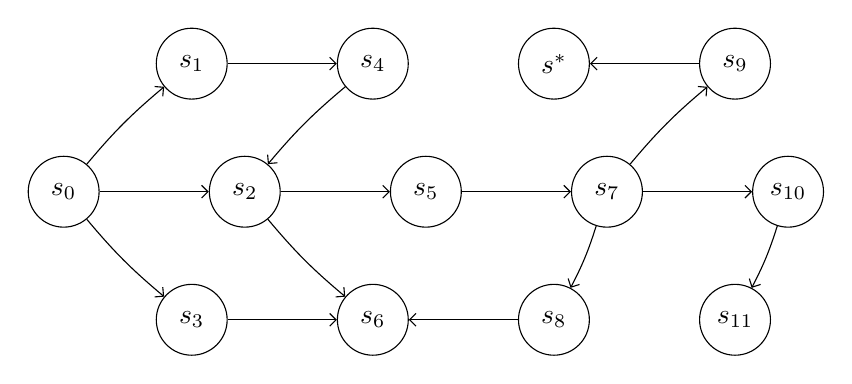
\begin{tikzpicture}[every node/.style={circle, draw}, node distance=23mm, minimum size=9mm]
        \node (s0) {$s_0$};
        \node[above right of=s0] (s1) {$s_1$};
        \node[right of=s0] (s2) {$s_2$};
        \node[below right of=s0] (s3) {$s_3$};
        \node[right of=s1] (s4) {$s_4$};
        \node[right of=s2] (s5) {$s_5$};
        \node[right of=s3] (s6) {$s_6$};
        \node[right of=s5] (s7) {$s_7$};
        \node[right of=s6] (s8) {$s_8$};
        \node[above right of=s7] (s9) {$s_9$};
        \node[right of=s7] (s10) {$s_{10}$};
        \node[right of=s8] (s11) {$s_{11}$};
        \node[left of=s9] (goal) {$s^*$};

        \draw[-Straight Barb] (s0) to (s2);
        \draw[-Straight Barb] (s0) to[bend left=5] (s1);
        \draw[-Straight Barb] (s0) to[bend right=5] (s3);
        \draw[-Straight Barb] (s1) to (s4);
        \draw[-Straight Barb] (s2) to (s5);
        \draw[-Straight Barb] (s2) to[bend right=5] (s6);
        \draw[-Straight Barb] (s3) to (s6);
        \draw[-Straight Barb] (s4) to[bend right=5] (s2);
        \draw[-Straight Barb] (s5) to (s7);
        \draw[-Straight Barb] (s7) to[bend left=5] (s8);
        \draw[-Straight Barb] (s7) to[bend left=5] (s9);
        \draw[-Straight Barb] (s7) to (s10);
        \draw[-Straight Barb] (s8) to (s6);
        \draw[-Straight Barb] (s9) to (goal);
        \draw[-Straight Barb] (s10) to[bend left=5] (s11);
      \end{tikzpicture}
\end{figure}

To illustrate, Figure~\ref{fig:statespace} presents a state space. BFS starts by expanding the initial state $s_0$ and then expands $s_1$, $s_2$, and $s_3$. In sequence, it expands the successor of $s_1$ ($s_4$), then of $s_2$ ($s_5$ and $s_6$), until a solution is found. On the other hand, DFS expands the initial state $s_0$ and continues expanding a newly generated successor until it reaches a solution or a state without successors (e.g., $s_6$ or $s_{11}$), at which point the algorithm backtracks to the nearest state that has an unexpanded successor and continues the search.

Blind search algorithms are unsuitable for solving planning tasks due to their lack of efficiency in exploring the state space, which is typically vast and contains numerous paths. Instead, heuristic search is used, which will be introduced in the next section. However, BFS and DFS can still be valuable in planning as sampling algorithms. By sampling the state space using these algorithms, we can selectively focus on regions either closer to the initial state, using BFS, or, more distant, using DFS.

\subsection{Heuristic Search}
\label{sec:background_heuristicsearch}

Exploring the state space systematically to find a plan can quickly become computationally infeasible for planning domains with large state spaces. Therefore, the primary approach for solving planning tasks is heuristic search. Heuristic search algorithms address this challenge by using heuristics to guide the search toward promising regions of the state space. These heuristics estimate how close a given state is to the goal state and guide which successors to prioritize during the search.

A commonly used heuristic search algorithm in classical planning is \astar search. \astar combines the cost of reaching a state from the initial state ($g$-value) with a heuristic estimate of the remaining cost to reach the goal state ($h$-value). By considering both the past cost and the estimated future cost, \astar can efficiently explore the state space to find the optimal solution, provided that the heuristic is admissible (does not overestimate the actual $h$-value).

Greedy Best-First Search (GBFS), another widely used heuristic search algorithm in classical planning, is a variant of \astar search that prioritizes expanding states with the lowest heuristic values without considering the past cost of reaching those states. Both \astar and GBFS are considered a ``greedy'' algorithm because it only considers the heuristic estimate and makes decisions solely based on that information. While GBFS can be highly efficient regarding exploration speed, it does not guarantee finding an optimal solution as \astar does. Nonetheless, GBFS is a popular choice in planning tasks where finding any feasible solution quickly is more important than finding the optimal solution. Therefore, in our experiments, GBFS serves as the search algorithm.

\subsubsection{Heuristic Functions}
\label{sec:background_heuristicfunctions}

Heuristic search algorithms require the use of a heuristic function. A heuristic function~$h:\mathcal{S}\rightarrow\R_{+}\cup\{\infty\}$ maps each state in the state space~$\mathcal{S}$ to a non-negative number or $\infty$. The number represents the cost-to-goal estimate ($h$-value) for the given state. An infinity value indicates a dead-end state, i.e., without any paths leading to the goal. A heuristic function is more efficient when its $h$-value closely approximates the actual goal distance. The optimal heuristic \hstar produces the cost of an optimal $s$-plan for all state~$s \in \mathcal{S}$.

The heuristic function has certain properties, such as admissibility, consistency, and goal-awareness. An admissibility heuristic function never overestimates the actual goal distance. It guarantees optimality when combined with specific search algorithms such as \astar. A heuristic function is consistent if, for every state $s \in \mathcal{S}$ and for every applicable operator $o$ with $s' = \sucs(s,o)$, it holds that $h(s) \leq cost(o) + h(s')$. Finally, a goal-aware heuristic guarantees $h(s) = 0$ for all goal states $s \subseteq s^*$.

Heuristics can be arbitrary functions, allowing for flexibility in designing based on domain knowledge and problem-specific insights. Therefore, a heuristic can be classified as model-based or model-free. In a model-free setting, we interact with the planning task only by functions that allow accessing the initial state~$s_0$, the goal condition~$s^*$, and the successors $\sucs(s)$ of a state $s$. In this setting, we do not have access to the logical description of operators; we only have access to black-box functions~\cite{Sturtevant2019} -- which could also be learned -- that, given a state, returns its successors and predecessors\mr{is that so? could be very costly, mostly not polynomial: there can be many preconditions; a more reasonable model allows to enumerate or sample them}. Note that this setting is also used in reinforcement learning.
% Some approaches\mr{give an example} also provide access to each variable's domain.
In contrast, a model-based heuristic uses the complete description of the model, which permits, for example, reasoning about operators and the computation of mutexes.

An example of a model-based heuristic is the FF~(Fast-Forward) heuristic~\cite{Hoffmann.Nebel/2001}, which computes its cost-to-goal estimates by considering a relaxed version of the planning problem. In a relaxed version, all effects that remove facts from a state (delete effects) of the operators are ignored, resulting in a simplified version of the problem. The FF heuristic extracts a solution from a relaxed version and computes the cost of operators in the plan, using it as the cost-to-goal estimate. As model-free, we have the goal-count heuristic, which does not rely on the planning model. Instead, it counts the number of unsatisfied goal conditions in the current state, assuming that each unsatisfied condition requires an additional unit cost operator to be satisfied. Both the FF and goal-count heuristics are addressed in our experiments~(Chapter~\ref{sec:experiments}).

\section{Neural Networks}
\label{sec:background_neuralnetworks}

Neural networks (NN) have gained popularity due to their ability to learn and generalize from datasets. In classical planning, various approaches using NNs have been proposed (see Section~\ref{sec:background_relatedwork}). These approaches range from simpler models that prioritize processing speed -- and, consequently, expansion rate -- to more complex architectures that exploit the relational structure of a domain.

\begin{figure}[ht]
    \caption{Structure of the artificial neuron.}
    \label{fig:neuron}
    \centering
    \includegraphics[width=0.8\linewidth]{figures/neuron.png} \\
    Source: Haykin~(\citeyear{Haykin/2009})\rvi{convert to pdf}
\end{figure}

Essentially, NNs are composed of multiple artificial neurons, whose structure is illustrated in Figure~\ref{fig:neuron}. A neuron~$k$ consists of four components: input signals~$x_1,\ldots,x_m$, weights~$w_{k1},\ldots,w_{km}$, bias term~$b_k$, and an activation function~$\varphi$. A neuron~$k$ produces an output~$y_k = \varphi(v_k + b_k)$ where $v_k = \sum_{j \in [m]} w_{kj} x_j$. The activation function introduces non-linearity to the output. One common example is the Rectified Linear Unit (ReLU) activation $\varphi(v) = max(0,v)$.

\begin{figure}
    \caption[Graph of a neural network.]{Graph of a neural network. Vertices and edges represent the neurons and their connections, respectively.}
    \label{fig:neuralnetwork}
    \addvspace{\baselineskip}
    \centering
    \includegraphics[width=0.9\linewidth]{figures/network.png} \\
    \addvspace{\baselineskip}
    Source: Haykin~(\citeyear{Haykin/2009})
    \rvi{convert to pdf}
\end{figure}

The NN comprises multiple layers of neurons, as illustrated in Figure~\ref{fig:neuralnetwork}, which transform the input data into an output. The input layer receives the input data and passes it to the subsequent layers. The hidden layers, located between the input and output layers, weigh the neuron weights to learn the features that transform the input data into the desired output. These hidden layers enable the network to capture complex patterns and relationships within the data. Finally, the output layer produces the prediction for the given input. A specific type of NN called Feedforward Neural Network (FNN) allows information to flow in one direction, from the input layer through the hidden layers to the output layer. When an NN has multiple hidden layers, usually more than two\rv{there is no consensus but it is common to find that, in general, more than two hidden layers is deep}, it is referred to as a deep neural network.

The learning process involves adjusting the network's parameters, such as weights and biases, to minimize the error between its predictions and the true values of the training samples. This adjustment is typically performed using an optimization algorithm to minimize a specified loss function. One commonly used loss function is the Mean Squared Error (MSE), which quantifies the error by calculating the mean squared difference between the predicted and true values. Training is often performed on batches of data rather than individual samples to update the parameters efficiently. The batch size determines the number of samples that are processed together before updating the network's parameters. Batches enable training with larger sets of samples, which can be computationally infeasible to handle all at once. Haykin (\citeyear{Haykin/2009}) provides further details for a more comprehensive understanding of weight adjustment and training in NNs.

By iteratively adjusting its parameters based on the training data, an NN gradually improves its ability to make accurate predictions. The quality of the NN depends on the quality and diversity of the sample set. Additionally, the network's capacity to learn and generalize from the training data is influenced by its architecture. Each one has its purpose and may excel in specific types of tasks. One example of such an architecture is the residual network.

\subsection{Residual Networks}
\label{sec:background_resnets}

ResNet, short for Residual Network, was proposed by He et al.~(\citeyear{He.etal/2016}) and has gained attention due to its ability to address the vanishing gradient problem~\cite{Hochreiter/1998} and improve training performance for deep NNs. While its initial success was in image recognition, ResNet has also been used in planning~\cite{Agostinelli.etal/2019,Ferber.etal/2022} to address training deep neural networks.

ResNet uses the concept of residual connections or skip connections, which enable the network to learn residual mappings. These connections allow the network to bypass specific layers and pass the input directly to deeper layers. By doing so, ResNet mitigates the vanishing gradient problem in deep networks, where the gradient becomes increasingly small as they propagate backward through the network layers, causing the weights in the earlier layers to update slowly or not at all. The residual connections establish ``highways'' for information flow, helping maintain the signal propagation.

\begin{figure}[t]
    \caption[A regular block and a residual block.]{A regular block (left) and a residual block (right).}
    \label{fig:residual_block}
    \addvspace{\baselineskip}
    \centering
    \includegraphics[width=0.75\linewidth]{figures/residual_block.pdf} \\
    Source: Zhang et al.~(\citeyear{Zhang.etal/2021})
\end{figure}

Figure~\ref{fig:residual_block} illustrates a schematic representation of both a regular block and a residual block -- with a shortcut connection that skips two layers -- in a ResNet architecture. In a regular block, the output of its layers is directly mapped to the activation function. On the other hand, in a residual block, the network needs to learn the residual mapping. Instead of forcing the network to learn all the information from the input, residual blocks allow it to focus only on the residual, i.e., the difference between the input and output, needed to achieve the desired output. He et al.~(\citeyear{He.etal/2016}) provide a more detailed explanation of ResNets.

\subsection{Learning Heuristic Functions}
\label{sec:background_learningheuristics}

Many heuristics for classical planning are derived from a model of the task, such as \sas. An obvious alternative is to learn to map a state~$s$ to its heuristic value~$h(s)$. We focus on learning with NNs, although other supervised learning methods could be used. To learn a heuristic function, an NN is trained on pairs of states~$s$ and cost-to-goal estimates~$c$. The learned heuristic functions are usually not admissible, so traditional optimality guarantees are lost.

A propositional representation of a state is more suitable for learning functions over states, as the variables in a planning task are categorical variables. To this end, consider a planning task $\Pi=\langle\mathcal{V},\mathcal{O},s_0,s^*, \text{cost}\rangle$, and let $\mathcal{V}=\{v_1,\ldots,v_n\}$ and $D(v_i)=\{d_{i1},\ldots,d_{i,s_i}\}$, $i\in[n]$ be some order of the variables and their domains. We represent any state $s$ by a sequence of facts $$\mathcal{F}(s)=(f_{11},f_{12},\ldots,f_{1,s_1},\ldots,f_{n1},f_{n2},\ldots,f_{n,s_n}),$$ where each fact $f_{ij}=[s(v_i)=d_{ij}]$ indicates if variable $v_i$ assumes value $d_{ij}$ in state $s$. Note that facts $\mathcal{F}_i=\{f_{i1},\ldots,f_{i,s_i}\}$ corresponding to variable $v_i$ satisfy the consistency condition $\sum_{f\in \mathcal{F}_i} f\leq 1$ since each variable assumes at most one value, and $\sum_{f\in \mathcal{F}_i} f=0$ only if $v_i$ is undefined. More generally, for any set of facts $\mathcal{F}$ we write $\mutex(\mathcal{F})$ if $\sum_{f\in \mathcal{F}} [f]\leq 1$ must be satisfied in states of $\Pi$. Many planning systems can deduce mutexes from the description of the planning task $\Pi$~\cite{Helmert/2009}; we will discuss and analyze their utility for sampling states later. Some architectures provide additional input to the neural network, e.g., the propositional representation of the goal condition. The target output for training may be the cost-to-goal estimates directly or some encoding of them.

An important aspect of sample generation related to challenges C1 and C2 (Chapter \ref{sec:intro}) is the degree of dependency on the domain model -- ideally, we would like to learn in a model-free setting -- or the planning task and the cost of generating the samples. The cost of sample generation depends on the number of samples and the cost to generate each. This generates the problem of deciding how many samples are required since, in general, only a very small part of the state space can be sampled. More importantly, ideal samples would be labeled with the optimal heuristic $h^*$. In general, ideal labeling is impractical since it requires solving the planning task on a large number of initial states. Therefore, we are mainly interested in good heuristic estimates that can be generated fast. We analyze the influence of sample size and quality experimentally later.

Additionally, and related to challenges C3 and C4, network architecture and sample generation depend on the range of tasks the learner intends to generalize. This may be the state space of a planning task, a planning domain, or an entire planning formalism. In the first case, the set of planning tasks is defined over any pair of initial state~$s_0$ and goal~$s^*$. Often the set of planning tasks is restricted to select the initial state from the FSS of some given initial state and to a fixed goal. In the second case, the learned function has to generalize over all domain tasks. Finally, a learning-based heuristic that generalizes over a planning formalism is domain-independent. An important aspect of sample generation is the distribution of states which are part of the sample set. For example, the sample set can contain only states with a short distance to the goal or only states with a short distance to the initial states. In this dissertation, the distribution of \hstar-values, e.g.,~in a histogram, represents the distribution of states in the sample set.

\section{Related Work}
\label{sec:background_relatedwork}

Two main research topics have been on learning heuristic functions: strongly and partially model-based approaches. The first one uses model description, such as information about preconditions and effects of operators, to generate samples or build the NN and aims to generalize over domains or a planning formalism. The second one uses limited access to the model only to identify mutexes, generating states close to those encountered during a search, and aims to generalize only over a state space.

\subsection{Strongly Model-Based}

The usual setting for the first set of approaches~\cite{Toyer.etal/2018,Shen.etal/2020,Toyer.etal/2020,Gehring.etal/2022,Stahlberg.etal/2022} is to train different architectures of NN with samples of small tasks of a domain generated with a strongly model-based method and evaluated on larger tasks of the same domain. These architectures can be general networks such as neural logic machines~\cite{Dong.etal/2018} and graph neural networks~\cite{Gori.etal/2005,Scarselli.etal/2008}.

In the context of planning, Shen et al.~(\citeyear{Shen.etal/2020}) introduced hypergraph neural networks (HGN) as an extension of graph networks~\cite{Battaglia.etal/2018}. HGN aims to learn planning heuristics through training, focusing on developing domain-independent heuristics capable of generalizing across various domains, as well as domain-specific and multi-domain heuristics. The HGN encompasses vertices representing task propositions within a hypergraph structure, with edges denoting operators connecting the preconditions to their effects.

Another approach proposed explicitly for planning tasks is the Action Schema Networks~(ASNet)~\cite{Toyer.etal/2018}. ASNets are composed of alternating proposition and action layers, with the first and last always being an action layer. Each action layer contains an action module for each operator in a specific task, while each propositional layer contains a proposition module for each fact in the task. Weight sharing is used to optimize efficiency, where action modules with operators derived from the same action schema share the same weight, and proposition modules with atoms derived from the same predicate share the same weight. This weight sharing allows for the reuse of a single set of learned weights across all tasks within a class of planning problems.

These networks achieve competitive results compared to logic-based heuristics and can generalize well, but require the logical description of the domain and the task to be instantiated. These approaches also help in understanding learning heuristics. For example, the main goal of St\aa hlberg et al.~(\citeyear{Stahlberg.etal/2022}) is to understand the expressive power and limitations of learning heuristics. The main limitation of these approaches is the strong dependence on the domain model and task description.

\subsection{Partially Model-Based}

The second set of approaches~\cite{Ferber.etal/2020a, Yu.etal/2020, Ferber.etal/2022, OToole/2022} typically trains an FNN and evaluates the learned heuristic on a state space using tasks with the same goal and different initial states. These networks are trained with pairs of states and cost-to-goal estimates. Ferber et al.~(\citeyear{Ferber.etal/2020a}) systematically study hyperparameters on the FNN and found that, for a fixed architecture, two aspects significantly influence how informed the heuristic is: the subset of selected samples and the size of the sample set.

Ferber et al.~(\citeyear{Ferber.etal/2022}) use a combination of backward and forward searches~\cite{Arfaee.etal/2011}. First, they generate new initial states with backward random walks and then solves them with a GBFS guided by a learned heuristic. The sampling is performed in parallel with the training. The number of samples per search varies throughout the process, starting with a random value ranging from $0$ to $5$ and doubling it as plans are found. The plans found provide the samples for the next training epoch, where each sample is a state in a plan with the cost-to-goal estimate as its distance to the goal through the plan. Their FNN architecture is a ResNet with two hidden layers and a residual block consisting of two more hidden layers.

O'Toole et al.~(\citeyear{OToole/2022}) use the same FNN architecture as Ferber et al.~(\citeyear{Ferber.etal/2022}), which is also applied in this dissertation. They use random walks to perform $5$ backward searches from the goal, with a depth of $500$, where the depth at which the state is generated serves as a cost-to-goal estimate. Each sampled partial state is then converted into $20$ complete states and added to the sample set. Furthermore, they sample an additional $50$\,K randomly generated states with a cost-to-goal estimate equal to the maximum value in the sample set plus one, resulting in a total of $100$\,K samples. They showed that random sampling improves the performance of the heuristic function by including in the sample set states from regions of the state space not reached by the backward search.

Yu et al.~(\citeyear{Yu.etal/2020}) used a backward search approach with the DFS algorithm. In their best configuration, they sample $100$\,K states in $500$ searches, i.e., $200$ states per search, with a cost-to-goal estimate equal to the depth at which the state was generated. In contrast to the previous approaches, they use a compact FNN consisting of only one hidden layer with $16$ neurons.

The methods from the partially model-based approaches are highly independent of the domain model and planning task description and require low computational resources to generate samples and train the FNN. However, despite having competitive results compared to logic-based heuristics, they can still not surpass the goal-count heuristic.

\chapter{Sample Generation}
\label{sec:sampling}

\rvi{WIP from here until the end of the chapter}

We aim to investigate sample generation systematically. Therefore, we focus on how three aspects of sample generation influence the performance of the learned heuristic to guide a search algorithm: the distribution of states $s_i$ in the state space part of the sample set, the quality of the estimates $h_i$ of samples with respect to the $\hstar$-value, and the methods that generate sample sets. In our setting, learning a heuristic function requires a set of samples $(s_1,h_1),\ldots,(s_N,h_N)$, where each sample $(s_i,h_i), i\in[N]$ consists of a state $s_i$ and a cost-to-goal estimate (or $h$-value) $h_i$.

We restrict our study to generalizing over planning tasks with initial states part of the same forward state space~(\fssp) and a fixed goal condition. We study model-free approaches with access to predecessors and successors of partial states through a black-box function, the goal condition, and the domain of each variable. We also study model-based approaches that have access to mutexes derived from a \sas model. We approach first, in Section~\ref{sec:generation}, the generation of states, and then, in Section~\ref{sec:hvalue}, the estimation of the cost-to-goal. In both sections, we discuss approaches from the literature and introduce new methods. The new methods are a novel sampling strategy combining regression by breadth-first search with random walk, an adaptive regression limit, and two improvement methods for cost-to-goal estimates.

\section{Generation of States}
\label{sec:generation}

Unlike other domains in machine learning, where datasets of samples are often collected in real-world experiments and need to be manually annotated and curated, sample generation here is an algorithmic problem since we have access to the state space and can compute cost-to-goal estimates. Approaches from the literature to generate the states include methods based on progression from one or more initial states, random sampling of the state space, or regression from the goal. In both progression and regression, one can apply different expansion strategies such as random walks, breadth- or depth-first searches, or teacher searches which include ``on policy'' searches in methods using reinforcement learning or bootstrapping~\cite{Arfaee.etal/2011}. A problem in progression and random sampling is obtaining the cost-to-goal estimates. Without access to efficiently computable heuristic functions, or in model-free approaches, these values have to be obtained by search, which can have a cost exponential in the size of the task. To remain less dependent on models than logic-based methods and also more general, we focus on regression for which an upper bound on the cost-to-goal is readily available, discussed in Sections~\ref{sec:sampling-generation}~and~\ref{sec:rollout-depth-limit}. Still, regression leads to partial states, so the problem of generating complete states is addressed in Section~\ref{sec:sample-completion}. Random sampling is also discussed in Section~\ref{sec:random-samples-theory}.

\subsection{Sampling by Regression}
\label{sec:sampling-generation}

To generate samples, we expand the backward state space through regression. We consider expansion by breadth-first search (\bfs) and depth-first search (\dfs), by random walks (\rw), as well as a combination of BFS with random walks explained below. A regression rollout is defined as a series of state expansions, and it stops if the last expanded state has no predecessors or is at the depth limit $L$. The sampling generation process stops if the number of required samples $N$ has been reached. Note that random walks can have multiple rollouts due to $L$, while \bfs and \dfs only have one -- except if the number of states in the backward state space is less than $N$, in which case they need to perform more than one rollout.

During expansion, we optionally use mutexes obtained from an analysis of the planning task -- in our case as computed by Fast Downward~\cite{Helmert/2006} -- to discard partial states which cannot be completed to complete states without violating a mutex, as described in Section~\ref{sec:sample-completion}. We also discard repeated partial states for random walk rollouts, such that a single rollout never cycles, although the same partial state may be sampled several times in different rollouts. Starting from $h(s^*)=0$, a state $s'\in\pred(s,o)$ obtained by applying an operator $o$ backwards to state $s$ has a cost-to-goal estimate $h(s')=h(s)+\text{cost}(o)$. We reset to $h(s)=0$ the cost-to-goal estimate for samples $s\subseteq s^*$ that satisfy the goal condition. States are added to the sample set when generated in the random walks and when expanded in BFS and DFS. In all methods, operators backward applicable to a state are applied in random order.

Different expansion strategies generate sample sets with varying frequencies of  optimal distances from the goal. In our experience, good coverage of states close to the goal, such as those obtained by BFS or random walks, is useful, as is the greater depth obtained by DFS or random walks. However, random walks from the goal often sample states close to the goal multiple times, and DFS can lead to a concentration of distant samples from the goal. Based on these observations, we propose a novel combination of BFS and random walks called \bfsrw that aims to have a good coverage close to the goal and a diverse set of samples from the remaining state space. \bfsrw has two phases. In the first phase, a fixed percentage $p_\bfsrw$ of the $N$ samples is generated by BFS. (Note that $p_\bfsrw$ can additionally represent time and memory limitations -- in this case, \bfs stops once either of them is reached first.) The \bfs expands a state from layer $k$ that generates $n$ states from layer $k+1$, and these states are sampled only if the current total samples plus $n$ are within $p_{\bfsrw}N$ samples; otherwise, no states are sampled and \bfs expands another state. Let $Q$ be the states of the set of samples that have not been expanded. The second phase generates multiple random walk rollouts, each starting from a state in $Q$ chosen randomly with a complete replacement only after all states have been selected once. This is repeated until reaching $N$ samples in the sample set. During a random walk, states sampled in the BFS phase are discarded.

\subsection{Maximum Regression Limit}
\label{sec:rollout-depth-limit}

A simple strategy to limit the expansion depth is to define some maximum limit $L$. This has been used in previous work, e.g.,~by \citeyear{Yu.etal/2020} and \citeyear{OToole/2022} with $L=200$ and $L=500$, respectively. A fixed limit is not the optimal choice for tasks with state spaces of different diameters or different maximum distances to a fixed goal when we aim for a representative sample of the state space. This is a problem in particular for regression: if the maximum regression limit $L$ overestimates the maximum distance-to-goal by much, the corresponding cost-to-goal estimates will be too large; if it underestimates it, samples may be concentrated too close to the goal.

Therefore, the most effective maximum regression limit for a fixed goal should be defined as a function of the longest distance \distfarthest from the goal state to any other potential initial state. For BFS, \distfarthest would be the ideal estimate; for DFS and random walks, higher limits are required since they do not follow the shortest paths. Since \distfarthest, in general, is unknown, we propose to define a maximum regression limit $L$ by two adaptive, approximated methods, according to the input task parameters, the first of which is model-free and the second model-based. The first is a regression limit that equals the number of facts $L=F=|\mathcal{F}(s_0)|$. The second is to set $L=\bar F=\ceil{\facts/\overline{\eff}}$ where $\overline{\eff}=\sum_{o\in \mathcal{O}} |\eff(o)|/|\mathcal{O}|$, i.e.,~the number of facts per mean number of effects in the operators.

\subsection{Sample Completion}
\label{sec:sample-completion}

Regression sampling generates a set of partial states, while the NN is trained on and receives as input complete states during the search. Each partial state can be completed by assigning a value $s(v)\in\dom(v)$ to all fact pairs $(v,s(v))$ where $s(v)=\bot$. Since it makes no assumptions except the domains, we consider this strategy model-free. We further study two stronger methods of generating complete states: a model-based one that uses mutexes and an ideal completion that only generates states that are reachable from the initial states of interest.

The model-based method also assigns a random value $s(v)\in\dom(v)$ to each undefined variable but excludes states that do not satisfy mutexes derived from the planning task. This is achieved by rejection sampling, where the undefined variables are processed in random order and set to a random value that does not violate the mutexes. If the state could not be completed in $10$\,K trial orders, we leave the facts undefined, i.e., set to false (zero)\footnote{Empirically this case is negligible since it occurs in about $0.1\,\%$ of the samples, in four of nine domains.}.

The model-based solution can still generate states that can never be reached during the search. To study the effect of generating only relevant states, we therefore also include an ideal state completion method. This method applies only to small tasks, where we can enumerate the complete forward state space \fssp of the initial state $s_0$. Then, to complete a partial state $s$ we sample a random state from $s~\cap$~\fssp. Since we sample by regression for some states $s~\cap$~\fssp may be empty; such states are discarded during regression.

\subsection{Randomly Generated Samples}
\label{sec:random-samples-theory}

\citeyear{OToole/2022} have shown that adding randomly generated samples to a set of samples generated by expansion improves the performance of the search algorithm guided by the learned heuristic. They propose to set the cost-to-goal estimate for randomly generated samples to $L+1$ for a maximum regression limit of $L$. To study the effect of randomly generated samples, we include this method in our study. These samples are generated from fully undefined states using the model-based technique described in the previous section. If the generated state $s$ is already part of the sample set, i.e.,~$s = s_i$ for some $i\in[N]$ it receives cost-to-goal estimate $h_i$, otherwise the cost estimate $1+\max_{i\in[N]} h_i$ that is larger than all samples estimates. For simplicity, from this point on we refer to ``randomly generated samples'' as ``random samples''.

\section{Improving Cost-to-Goal Estimates}
\label{sec:hvalue}

We start by observing that cost-to-goal estimates never underestimate the true cost-to-goal $h^{*}$, as follows.

\begin{property}
    \label{prop:hvalue}
    The cost-to-goal estimate $h(s)$ of a sample $s$ obtained by regression satisfies $h(s)\geq h^*(s)$.
\end{property}
\begin{proof}
    This follows simply because each estimate is witnessed by a plan. As observed in Section~\ref{sec:background}, a valid regression sequence $\rho=(o_1,\ldots,o_k)$ generates a sequence of partial states that can reach the goal in at most $k$ steps and with cost at most $\sum_{i\in[k]}\text{cost}(o_i)$, which cannot be lower than the optimal cost.
\end{proof}

In general, we expect better $h$-value estimates to lead to better-learned heuristics, and in turn to less expanded states during a search, although this is not necessarily the case \cite{Holte/2010}. Therefore, we apply two simple procedures that improve the cost-to-goal estimates but maintain \cref{prop:hvalue}. The first, dubbed \hmin, minimizes estimates over repeated samples, and the second, \hvfc, over successors of samples.

\subsection{Improvement of Repeated Samples}
\label{sec:hmin}

In most state spaces, it is common for a state to be sampled in more than one random walk rollout, ending up with multiple duplicates with different estimates. Thus, for all sampled states $s$ we update each cost-to-goal estimate to the best estimate $h(s) = \min\{h_i \mid s=s_i, i\in[N]\}$. Since different partial states can generate identical complete states, the improvement is applied to partial states as well as complete states. We call this procedure \emph{sample improvement} (\hmin). Choosing the minimum $h$-value is clearly sound since, in all cases, we have valid plans from a regression that witness these distances; for the same reason, \cref{prop:hvalue} still holds.

\subsection{Improvement over Successors}
\label{sec:hvfc}

Besides sampling the same states, it is common to sample states that are neighbors in the state space, particularly for states close to the goal. This can be used to improve the cost-to-goal estimates, as follows. Consider a directed graph $G=(V,A)$ over all sampled partial states, i.e.,~$V=\{s_i\mid i\in[N]\}$. For every pair of states $s,t\in V$ such that for some operator $o\in\mathcal{O}$ applicable to $s$ we have $\sucs(s,o)\subseteq t$, we add an arc $(s,t)$ of length $\text{cost}(o)$ to $A$. (Unlike in regression, if $\pre(o)$ mentions an undefined variable in $s$ then $o$ is not applicable.) For fast subset, we keep all samples in a trie and search for each successor in the states that are supersets. For partial states generated by regression, by construction, at least one such successor exists, except for the goal state $s^*$. We then compute the shortest paths to the goal in graph $G$ (e.g.,~via the Dijkstra algorithm), and update the cost-to-goal estimates with these distances. We call this procedure \emph{successor improvement} (\hvfc). As for \hmin, all distances are witnessed by plans, so \cref{prop:hvalue} is maintained.

\section{Example}
\label{sec:example}

%Check the example of Fukunaga. We need: a small example that is able to demonstrate all techniques: regression, partial states, minimization, \bfs, random walks, etc.

\chapter{Experiments}
\label{sec:experiments}

In this section, we present two sets of experiments. In the first set, we analyze the behavior of sampling methods on planning tasks for which we can enumerate the complete state space with associated optimal cost-to-goal estimates \hstar. We study how different sampling methods influence the quality of the learned heuristic concerning the number of state expansions by a search algorithm. In the second set, we evaluate how our findings generalize to a practical setting with large planning tasks. Our methods are then compared to logic-based heuristics.

\section{Settings}
\label{sec:exp_settings}

We use a residual neural network~\cite{He.etal/2016} to learn a heuristic for a state space. The network's input is a Boolean representation of the states, where a fact is set to~$1$ if it is true in the state and~$0$ otherwise, as explained in Section~\ref{sec:background_learningheuristics}, and its output is a single neuron with the predicted $h$-value. The network has two hidden layers followed by a residual block with two hidden layers. Each hidden layer has~$250$ neurons that use ReLU activation and are initialized as proposed by He et al.~(\citeyear{He.etal/2015}). The training uses the Adam optimizer~\cite{Kingma.Ba/2015}, a learning rate of $10^{-4}$, an early-stop patience of~$100$, and a MSE loss function. Due to better results in preliminary experiments, we use batch sizes of $64$ for small and $512$ for large state spaces, and $90\,\%$ of the sampled data as the training set, with the remaining $10\,\%$ as the validation set. In the experiments, different learned heuristics are denoted as $\hat h_A$, where $A$ indicates different algorithmic choices.

We select the domains and tasks from Ferber et al.~(\citeyear{Ferber.etal/2022}), namely: Blocks, Depot, Grid, N-Puzzle, Pipes-NT, Rovers, Scanalyzer, Storage, Transport, and VisitAll. All domains have unit costs except for Scanalyzer and Transport, for which we consider the variant with unit costs. All methods are implemented on the Neural~Fast~Downward planning system with PyTorch~1.9.0~\cite{Ferber.etal/2020a,Paszke/2019}. Our source code, planning tasks, and experiments are available\footnote{Available at \url{https://github.com/bettker/NeuralFastDownward}}. All experiments were run on a PC with an AMD Ryzen~9 3900X processor, using a single core with $4$~GB RAM per process. We solve all tasks with \gbfs guided by the learned heuristic~\hnn with the lowest generation order as a tie-breaking strategy.

We note that an NN may fail to train if, after initialization, it outputs zero for all training samples (this is called ``born dead'' in Lu et al.~(\citeyear{Lu.etal/2020})). We noticed this occurs with a non-negligible frequency in experiments on smaller state spaces with fewer samples. Thus, we test for this condition, and if, after initialization, the network outputs zero for all samples in the training set, we reinitialize with a different seed until the network outputs a non-zero value for some sample.

We compare the experiments to a baseline \hnnbase with a similar configuration to previous approaches from the literature presented in Section~\ref{sec:background_relatedwork}. For the baseline, the NN is trained by a sampling method that uses random walks with a regression limit of~$200$ backward steps. In addition, mutexes are used during regression and for sample completion, but resetting the $h$-value to $0$ in goal states and the improvement strategies SAI and SUI are turned off. In preliminary experiments sampling with the FSM algorithm, we use $p_{\bfsrw}\in\{0.01,0.05,0.1,0.2,\ldots,0.9\}$. $p_{\bfsrw}=0.1$ achieved the best average performance. Thus, we fix $p_{\bfsrw}$ to this value in the experiments.

\section{Small State Spaces}
\label{sec:experiment1}

In this section, we study the behavior of different sampling methods on small state spaces. For each domain, we select the task with the largest size state space that can be enumerated completely to obtain \hstar-values. We only select tasks with state spaces with $30$\,K states or more, and fewer than $1$\,M states. Table~\ref{tab:small-instances} shows the tasks and their state space sizes. For domains Grid, Rovers, Scanalyzer, and Transport, the task had fewer than $30$\,K states, and VisitAll more than $1$\,M, so we manually modified these tasks. We could not find a task within our limits for Depot, Pipes-NT and Storage, so they were excluded from our experiments.
We generate the initial states for the small state spaces by performing a random walk of length~$200$ from the original initial state of a task. Rovers, Scanalyzer and VisitAll had duplicated initial states or that satisfied the goal state. Thus, for these domains, we generate the initial states with random walks of length $25$, $50$, and $8$, respectively.

\begin{table}[ht]
\centering
\begin{tabular}{llrllr}
   \toprule
    Domain & Task & \#States & Domain & Task & \#States \\ 
    \midrule
    Blocks & blocks-7-0 & 65990 & Scanalyzer & p03$^*$ & 46080  \\
    Grid & prob01$^*$ & 452353 & Transport & p02$^*$ & 637632  \\
    N-Puzzle & prob-n3-1 & 181440 & VisitAll & p-1-4$^*$ & 79931  \\
    Rovers & p03$^*$ & 565824 & & & \\ 
   \bottomrule
\end{tabular}
\caption{Size of the forward state spaces for the selected small tasks in seven domains. Tasks marked with~$*$ were modified.} 
\label{tab:small-instances}
\end{table}


In small state space experiments, the coverage for all methods is $100\,\%$. Therefore we use the number of expanded states to evaluate the quality of the heuristic function. In these experiments, we report means over experiments with five different network seeds, five different sample seeds, and $50$ initial states. The training time has been limited to $30$ minutes. If not stated otherwise, methods \bfs, \dfs, \rw, and \bfsrw use mutexes, the improvement strategies SAI and SUI, and the number of samples is equal to $1\%$ of the state space size. After initialization, the percentage of networks that output $0$ for all samples was at most $40\,\%$ (in Blocks), and all networks successfully passed the initialization test after the second initialization. Under these conditions, less than $1.5\,\%$ of the NNs did not converge within the time limit.

\subsection{Distribution of States}
\label{sec:experiment1-subset}

Our first set of experiments aims to analyze the influence of the distribution of sampled states in the state space on the quality of the learned heuristics. For this, we compare different sample generation algorithms, regression limits, random sample percentages, and state completion. If not stated otherwise, for the parameters that are not varied, we use the baseline setting defined above (regression limit $L=200$,  mutexes, no cost-to-goal improvement methods).

\subsubsection{Sample Generation Algorithms}

In this experiment, we compare four sample generation algorithms: \bfs, \dfs, \rw, and \bfsrw. To control the effect of the cost-to-goal estimates on the quality of the learned heuristic, we replace sample estimates with optimal values $h^{*}$ before training. Table~\ref{tab:small-h-optimal} shows the number of expanded states of a \gbfs guided by the learned heuristics and the mean $h^{*}$-values over the sampled states. We see that heuristic \hnnbfs leads to more expanded states than \hnndfs, which in turn expands about $50\,\%$ more states than \hnnrw and \hnnbfsrw, which perform similarly. Using \hnnbfs is significantly worse and leads to the highest or close to the highest number of expansions in all domains. Heuristic \hnndfs has a high number of expansions in Blocks, N-Puzzle, and Transport. Looking at the mean $h^{*}$-values, we see that samples generated by \bfs have the lowest, and those by \dfs the highest mean estimates in all domains. Although the distribution of \dfs is closest to that of the whole state space (inferred from the mean $h^{*}$-values), the resulting heuristic expands more states than \rw and \bfsrw, which generate states closer to the goal. Therefore, multiple random walk rollouts seem better than a single rollout with \bfs or \dfs due to increased sample diversity in different portions of the state space, covering states more likely to be visited during the search.

\begin{table}[ht]
\caption[Comparison of sampling strategies on $h^*$-values.]{Comparison of sampling strategies \bfs, \dfs, \rw, and \bfsrw on $h^*$-values. Expanded states of \gbfs with learned heuristics, and mean \hstar-values over the entire forward state space and the generated sample sets.}
\label{tab:small-h-optimal}
\addvspace{\baselineskip}
\centering
\begin{tabular}{lrrrrrrrrr}
           & \multicolumn{4}{c}{Expanded states} & \multicolumn{5}{c}{Mean $h^*$-values}                              \\
\cmidrule(lr){2-5}\cmidrule(lr){6-10}
Domain     & \hnnbfs  & \hnndfs & \hnnrw & \hnnbfsrw & \fssp & \bfs  & \dfs  & \rw   & \bfsrw \\
\midrule
% Blocks     & 5047.06  & 85.87   & 44.36  & \textbf{37.34}     & 18.77 & 10.77 & 17.68 & 11.93 & 14.42  \\
% Grid       & 112.68   & 122.36  & \textbf{99.25}  & 110.27    & 16.59 & 5.32  & 17.11 & 7.22  & 8.86   \\
% N-Puzzle   & 1477.23  & 176.83  & 109.47 & \textbf{109.17}    & 21.97 & 10.42 & 20.17 & 20.02 & 19.78  \\
% Rovers     & 12.87    & 13.09   & \textbf{11.82}  & 11.84     & 6.45  & 2.34  & 5.19  & 4.95  & 4.99   \\
% Scanalyzer & 175.93   & 25.54   & \textbf{24.46}  & 24.92     & 8.34  & 2.91  & 7.91  & 7.07  & 6.51   \\
% Transport  & 135.10   & 44.98   & 19.55  & \textbf{19.22}     & 12.23 & 2.94  & 11.30 & 10.05 & 9.52   \\
% VisitAll   & 53.28    & 21.98   & 19.19  & \textbf{18.72}     & 8.97  & 2.00  & 9.10  & 6.80  & 6.57   \\
%   \midrule
% Geo.~mean  & 201.93   & 48.31   & 33.98  & 33.54     & 12.21 & 4.22  & 11.45 & 8.81  & 9.09   \\
Blocks     & 5047.1  & 85.9   & 44.4  & \textbf{37.3}     & 18.8 & 10.8 & 17.7 & 11.9 & 14.4  \\
Grid       & 112.7   & 122.4  & \textbf{99.2}  & 110.3    & 16.6 & 5.3  & 17.1 & 7.2  & 8.9   \\
N-Puzzle   & 1477.2  & 176.8  & 109.5 & \textbf{109.2}    & 22.0 & 10.4 & 20.2 & 20.0 & 19.8  \\
Rovers     & 12.9    & 13.1   & \textbf{11.8}  & 11.8     & 6.4  & 2.3  & 5.2  & 5.0  & 5.0   \\
Scanalyzer & 175.9   & 25.5   & \textbf{24.5}  & 24.9     & 8.3  & 2.9  & 7.9  & 7.1  & 6.5   \\
Transport  & 135.1   & 45.0   & 19.6  & \textbf{19.2}     & 12.2 & 2.9  & 11.3 & 10.0 & 9.5   \\
VisitAll   & 53.3    & 22.0   & 19.2  & \textbf{18.7}     & 9.0  & 2.0  & 9.1  & 6.8  & 6.6   \\
  \midrule
Geo.~mean  & 201.9   & 48.3   & 34.0  & 33.5     & 12.2 & 4.2  & 11.4 & 8.8  & 9.1   \\
\end{tabular}
\end{table}


We now compare these results to results shown in Table~\ref{tab:small-h-estimate}, obtained on exactly the same states but using the cost-to-goal estimates obtained during sampling for training the NN. Note that the results for \bfs with estimated costs to the goal differ from those with exact values in Table~\ref{tab:small-h-optimal}. This happens because, during regression with \bfs, the cost-to-goal estimates are only exact on partial states; when turning them to complete states, the estimates can be larger than \hstar. Thus \hnnbfs with the estimates obtained during regression is less informed.

We can see that the relative order of the methods concerning the number of expanded states remains the same, although all methods expand more states. The increase in the number of expanded states is highest for \hnndfs, which expands about seven times more states. In contrast, the other methods expand about twice, meaning that the estimates produced by \dfs during regression are inferior to those produced by the other methods. The mean $h$-values confirm this: we can see that DFS significantly overestimates the true distances. Although \bfs has an estimation quality close to \hstar-value, its expanded states also degrade. These results suggest that sampling more states in localized regions of the state space (\bfs closer to the goal and \dfs more distant) is insufficient to achieve good results during the search with \gbfs.
Furthermore, \hnnbfsrw expands fewer states than \hnnrw and is the best in five of seven domains. Because \hnnbfsrw had a lower increase in expansions compared to \hnnrw, we focus on \bfsrw in the remaining experiments.

\begin{table}[ht]
\centering
\setlength{\tabcolsep}{1.19ex}
\begin{tabular}{lrrrrrrrrr}
\toprule
           & \multicolumn{4}{c}{Expanded states} & \multicolumn{5}{c}{Mean $h$-values}                                 \\
\cmidrule(lr){2-5}\cmidrule(lr){6-10}
Domain     & \hnnbfs   & \hnndfs & \hnnrw & \hnnbfsrw & \fssp & \bfs  & \dfs   & \rw   & \bfsrw \\
\midrule                                                                                
Blocks     & 5047.06   & 205.59  & 87.00  & \textbf{80.76}     & 18.77 & 10.77 & 166.11 & 28.09 & 38.43  \\
Grid       & 431.21    & 4102.36 & \textbf{263.56} & 276.23    & 16.59 & 6.77  & 184.59 & 21.06 & 22.46  \\
N-Puzzle   & 1477.23   & 1092.51 & 237.64 & \textbf{177.12}    & 21.97 & 10.42 & 187.51 & 96.29 & 90.65  \\
Rovers     & 91.82     & 27.76   & 21.89  & \textbf{18.85}     & 6.45  & 4.65  & 27.11  & 25.90  & 24.91  \\
Scanalyzer & 328.03    & 263.53  & 70.62  & \textbf{53.59}     & 8.34  & 2.98  & 146.17 & 90.30  & 87.86  \\
Transport  & 215.09    & 1321.10 & \textbf{110.98} & 130.14    & 12.23 & 3.27  & 196.12 & 95.20  & 88.59  \\
VisitAll   & 170.45    & 44.58   & 21.99  & \textbf{21.51}     & 8.97  & 2.74  & 28.48  & 22.48 & 22.37  \\ 
\midrule
Geo.~mean  & 446.72    & 326.66  & 79.78  & 73.12     & 12.21 & 5.14  & 103.50  & 43.30  & 44.38  \\     
\bottomrule
\end{tabular}%
\caption{Comparison of sampling strategies \bfs, \dfs, \rw, and \bfsrw on estimated $h$-values. Expanded states of \gbfs with learned heuristics, and mean $h$-values over the entire forward state space (FS) and the generated sample sets.}
\label{tab:small-h-estimate}
\end{table}


\subsubsection{Maximum Regression Limit}

In this experiment, we analyze the influence of the regression limit on the number of expanded states of sample generation strategy \bfsrw. We compare a fixed regression limit of $L=200$ to setting the regression limit to the number of facts $F$, or the number of facts divided by the mean number of effects $\bar F$. Values $F$ and $\bar F$ for the selected tasks, and additionally the largest distance of any state from the goal state~\distfarthest, are shown in Table~\ref{tab:small-strategies-limits}. Both $F$ and $\bar F$ overestimate the largest distance \distfarthest, except for $\bar F$ in three domains (namely Blocks, Scanalyzer, and VisitAll). As discussed in Section~\ref{sec:rollout-depth-limit} this is desirable since random walk rollouts do not follow the shortest paths.

\begin{table}[ht]
\caption[State space information and expanded states with different regression limits.]{State space information and expanded states of \gbfs guided by \hnn trained on \bfsrw samples with different regression limits and no $h$-value improvements. \distfarthest is the distance of the state most distant from the goal state.}
\label{tab:small-strategies-limits}
\addvspace{\baselineskip}
\centering
\begin{tabular}{lrrrrrr}
Domain     & \distfarthest & $F$ & $\bar F$ & \default          & \facts            & \meanfx        \\
\midrule
Blocks     & 24            & 64  & 17       & 80.76          & \textbf{58.06} & 185.00          \\
Grid       & 32            & 76  & 44       & 276.23         & 316.51         & \textbf{204.89} \\
N-Puzzle   & 31            & 81  & 41       & 177.12         & 104.52         & \textbf{80.83}  \\
Rovers     & 19            & 32  & 27       & 18.85          & 17.74          & \textbf{16.50}  \\
Scanalyzer & 15            & 42  & 20       & \textbf{53.59} & 57.02          & 88.76           \\
Transport  & 17            & 66  & 35       & 130.14         & 82.35          & \textbf{58.13}  \\
VisitAll   & 15            & 31  & 17       & \textbf{21.51} & 25.61          & 29.96           \\
\midrule
Geo. mean  &               &     &          & 73.12          & 63.36          & 69.48           \\
\end{tabular}
\end{table}


The right-hand side of Table~\ref{tab:small-strategies-limits} gives the number of expanded states for the three settings of $L$. We see that limits $F$ and $\bar F$ perform better than the fixed limit $200$, with $F$ best on one, $\bar F$ on four, and $200$ on two tasks. Also, when a limit of $200$ is best, the limit $F$ presents the closest results, but when $F$ or $\bar F$ are best, a limit $200$ can be much worse. Note that $F$ is the best only in the domain where $\bar F$ underestimates \distfarthest. To validate this, we set $L=\ceil{c\bar F}$ for $c\in\{1.25,1.5,2,2.5,3,3.5\}$ in an additional experiment on domain Blocks. The number of expanded states decreases to $c=3$ with a mean of $52.31$ expansions. Overall, the adaptive limits $F$ and $\bar F$, although imperfect, are better estimates of the best regression limit.

\subsubsection{Randomly Generated Samples}

In this experiment, we evaluate the effect of adding randomly generated samples to the sample set, as explained in Section~\ref{sec:random-samples-theory}. We generate sample sets $S=\{(s_1,h_1),\ldots,(s_N,h_N)\}$ where $10\,\%, 20\,\%,\ldots,100\,\%$ are random samples (to which the improvement strategies SAI and SUI are not applied) and the rest is sampled with \bfsrw and a regression limit $\bar F$. Random samples get an $h$-value of $H+1$ where $H=\max_{i\in[N]} h_i$ is the largest $h$-value in samples $S$, except when they are part of the samples, in which case they receive the corresponding estimate (this happens in fewer than $1\,\%$ of the states). Note that when using $100\,\%$ of random samples, each has the cost-to-goal estimate equal to the regression limit $L+1$ instead of $H+1$, as we do not have samples in $S$.

\begin{table}[tbp]
\centering
\begin{tabular}{lrrrrrrrr}
\toprule
           & \multicolumn{8}{c}{Percentage of random samples} \\
  \cmidrule(lr){2-9}
Domain     & 0      & 10    & 20    & 30    & 40    & 50    & 60    & 70      \\
\midrule
Blocks     & 177.88 & 59.23 & 57.00  & 63.75 & 63.25 & \textbf{48.99} & 65.26 & 74.47 \\
Grid       & 124.89 & \textbf{60.77} & 66.52 & 79.81 & 64.33 & 66.87 & 75.92 & 115.44 \\
N-Puzzle   & 89.47  & 87.60  & \textbf{80.93} & 88.76 & 86.64 & 81.62 & 89.38 & 96.26 \\
Rovers     & 17.03  & 14.16 & \textbf{13.45} & 13.63 & 13.60  & 14.34 & 14.23 & 16.38 \\
Scanalyzer & 55.29  & 37.88 & \textbf{28.34} & 33.74 & 32.37 & 42.94 & 28.85 & 35.83 \\
Transport  & \textbf{22.90}   & 24.58 & 25.95 & 27.44 & 33.02 & 34.53 & 43.36 & 52.36 \\
VisitAll   & 30.90   & 22.70  & \textbf{21.78} & 22.05 & 22.11 & 23.11 & 24.45 & 25.75 \\
\midrule
Geo. mean & 53.91 & 36.97 & 35.13 & 38.51 & 37.95 & 38.76 & 40.94 & 48.75 \\
\bottomrule
\end{tabular}
\caption{Expanded states of \gbfs with a learned heuristic over samples generated by \bfsrw with regression limit $\bar F$, all cost-to-goal improvement strategies, and a varying percentage of randomly generated samples.}
\label{tab:small-contrasting}
\end{table}


Table~\ref{tab:small-contrasting} shows the performance up to $70\,\%$ random samples. We have omitted the larger values since expansions are higher (namely $56.10$, $73.94$, and $11397.79$). The number of expansions is considerably reduced when using random samples, with $20\,\%$ random samples performing slightly better than other percentages. This also holds for individual domains, except Transport which expands on average a few states more, and N-Puzzle and Rovers, which expand a few states less.

To better understand the effect of random samples, we have performed three additional experiments with $20\,\%$ of random samples. The first focuses on cost-to-goal estimates. We keep the samples but replace $H+1$ with small values: a random $h$-value from the sample set $S$ or a random value drawn from $U[1,5]$. This leads to overall means of $295.65$ and $3832.14$ expanded states, respectively. The second experiment changes the distribution of the random samples: we force them to be part of the FSS. This leads to a mean of $36.90$ expanded states. Finally, the third experiment does not apply mutexes, leading to a mean of $36.11$ expanded states. From these additional experiments, it is clear that the most relevant factor is a high $h$-value, and the distribution and quality of the states seem to matter less. Overall, the most probable explanation for the effect of random samples seems to be that they help to increase the probability that the search is guided towards samples for which the network has learned good estimates, i.e., the samples obtained through regression.

\subsubsection{State Completion}

Now we focus on how sampled partial states are converted to complete states. In this experiment, all the samples have optimal cost-to-goal estimates \hstar. We compare three different sample completion strategies for a partial state $s$. All of them select a random state from the set of states represented by $s$ or a restriction of it: the set equals either to all states in $s$ (no restrictions), only those states that satisfy mutexes, or only states from the forward state space (perfect baseline).

Table~\ref{tab:small-estimates-mutex} presents the expanded states for these approaches. We can see that applying mutexes has a moderate effect and is very close to an ideal completion of the states. However, completing randomly also presents competitive results, except for N-Puzzle. Also, N-Puzzle with both restrictions should have similar results -- as for this particular domain, all partial states completed respecting the mutexes are part of the FSS~--, but this is not the case, as N-Puzzle is a particularly noisy domain with a high standard deviation of state expansions, aggravated by \gbfs. To verify this, we ran $900$ experiments ($30$ sample seeds and $30$ network seeds) for N-Puzzle ``Mutex'' and ``FSS'', and we achieved similar mean expansions of $84.4$ and $88.66$, respectively.

\begin{table}[ht]
\centering
\begin{tabular}{lrrr}
  \toprule
           & \multicolumn{3}{c}{Restriction} \\
  \cmidrule(lr){2-4}
Domain     & None   & Mutex  & \fssp         \\
\midrule
Blocks     & 212.30 & 207.18 & \textbf{190.96}        \\
Grid       & 104.34 & 96.02  & \textbf{87.80}         \\
N-Puzzle   & 225.62 & \textbf{79.42}  & 98.71         \\
Rovers     & 11.50  & 11.74  & \textbf{10.65}         \\
Scanalyzer & \textbf{41.20}  & 43.98  & 44.61         \\
Transport  & 17.98  & 17.86  & \textbf{16.65}         \\
VisitAll   & \textbf{22.17}  & 22.44  & 22.78         \\ 
\midrule
Geo.~Mean  & 51.37  & 44.15  & 43.57         \\ 
\bottomrule
\end{tabular}%
\caption{Expanded states of \gbfs with \hnn trained with \bfsrw, \meanfx, \hstar cost-to-goal estimates, and different state completion approaches.}
\label{tab:small-estimates-mutex}
\end{table}


\subsection{Estimates of Cost-to-Goal}

Our second set of experiments aims to analyze how techniques used to improve cost-to-goal estimates influence sample quality. To this end, we directly compare the difference of the improved estimates to \hstar-values. Then, to see how well the learned heuristics generalize, we evaluate them over the forward state spaces from Table~\ref{tab:small-instances}.

\subsubsection{Quality of Estimates}

First, we compare the quality of the cost-to-goal estimates to \hstar with and without $h$-value improvement techniques and distinct regression limits, as shown in Table~\ref{tab:small-samples-ssp}. This table shows the mean absolute difference between the sample estimates and \hstar, so smaller means indicate better approximations. Note that we are not evaluating the output of an NN but the estimates part of the sample set.

\begin{table}[ht]
\caption[Mean difference of the cost-to-goal estimates to \hstar.]{Mean difference of the cost-to-goal estimates of samples of the sample set to \hstar.}
\label{tab:small-samples-ssp}
\addvspace{\baselineskip}
\centering
\begin{tabular}{lrrrrrrr}
   & \multicolumn{3}{c}{No improvements} & \multicolumn{4}{c}{With \hmin and \hvfc}       \\
\cmidrule(lr){2-4}\cmidrule(lr){5-8}
Domain     & \default & \facts & \meanfx & \default & \facts & \meanfx \\
\midrule
Blocks     & 24.01    & 12.90  & 0.91    & 12.56    & 6.90   & \textbf{0.18}    \\
Grid       & 13.60    & 13.29  & 9.84    & 1.32     & 1.32   & \textbf{0.61}    \\
N-Puzzle   & 70.87    & 21.80  & 6.10    & 60.79    & 19.18  & \textbf{5.11}    \\
Rovers     & 19.92    & 11.58  & 9.74    & 6.70     & 5.29   & \textbf{4.88}    \\
Scanalyzer & 81.35    & 15.07  & 6.09    & 20.16    & 5.59   & \textbf{1.89}    \\
Transport  & 79.06    & 23.42  & 10.98   & 24.59    & 5.98   & \textbf{2.44}    \\
VisitAll   & 15.80    & 9.07   & 4.58    & 5.64     & 4.06   & \textbf{2.15}    \\
\midrule
Geo.~mean  & 33.45    & 14.56  & 5.56    & 10.95    & 5.35   & 1.60     \\
\end{tabular}
\end{table}

The improvement strategies SAI and SUI substantially reduce the estimates for all regression limiting methods. For \default, \facts and \meanfx, using only SAI reduces the estimates to $31.28$, $13.95$, and $4.93$, respectively, and using only SUI reduces the estimates to $11.1$, $5.48$, and $1.93$ respectively. Thus, SUI has the most effect on improving the cost-to-goal estimates compared to SAI.
Also, the adaptive regression limiting methods are superior to the fixed default \default, and \meanfx has the best results. When comparing \default to \meanfx without $h$-value improvements, the cost-to-goal estimate difference to \hstar decreases by about $6$ times on geometric mean. Blocks has the best performance, improving more than $25$ times. Finally, using both $h$-value improvements and \meanfx reduces the difference to \hstar from $33.45$ to only $1.60$.

\subsubsection{Evaluation Over the Forward State Spaces}

We now analyze the quality of our learned heuristics and the logic-based heuristics fast-forward \hff~\cite{Hoffmann.Nebel/2001} and goal-count \hgc over all states from the FSS of each task. Table~\ref{tab:small-strategies-sp-error} shows the results. Except for \hnnbase (baseline), the samples are generated with \bfsrw limited by \default, \facts or \meanfx, and improved with SAI and SUI. The learned heuristic \hnnrs is the same as \hnnbfsrwl{\meanfx}, but $20\,\%$ of the samples are randomly generated. We see that \hnnbfsrwl{\meanfx} reduces the difference of the predicted result to the real one by about $11$ times when compared to \hnnbase, and when compared to \hgc, it has the smallest difference in all but two domains. Also, \hnnbfsrwl{\meanfx} presents a similar mean difference to \hff. Due to the randomly generated samples in the sample set, \hnnrs doubles the difference compared to \hnnbfsrwl{\meanfx}, with a smaller value only in Blocks.

\begin{table}[ht]
\caption[Mean difference of heuristics to \hstar when evaluated over the \fssp.]{Mean difference of \hff, \hgc and \hnn, to \hstar when evaluated over the \fssp.}
\label{tab:small-strategies-sp-error}
\addvspace{\baselineskip}
\centering
\begin{tabular}{lrrrrrrr}
Domain & \hff & \hgc & \hnnbase & \hnnbfsrwl{\default} & \hnnbfsrwl{\facts} & \hnnbfsrwl{\meanfx} & \hnnrs \\
\midrule
Blocks       & 6.76 & 13.37 &  26.46  & 16.58 & 9.84  & 2.91 & \textbf{2.42} \\
Grid         & 3.72 & 13.78 &  26.85  & 4.21  & 4.10  & \textbf{2.73} & 9.78   \\
N-Puzzle     & \textbf{4.19} & 14.86 &  79.84  & 65.37 & 23.90 & 6.75 & 12.73   \\
Rovers       & \textbf{0.17} & 3.31  &  11.08  & 3.18  & 3.04  & 2.98 & 6.35   \\
Scanalyzer   & 2.78 & \textbf{1.08}  &  106.37 & 27.60 & 11.45 & 2.99 & 9.01   \\
Transport    & \textbf{1.13} & 8.63  &  109.77 & 33.53 & 12.54 & 7.05 & 14.89   \\
VisitAll     & \textbf{1.31} & 3.03  &  21.55  & 7.50  & 5.56  & 2.21 & 4.74   \\ \midrule
Geo. mean    & 1.84 & 5.92  &  39.80  & 13.91 & 8.13  & 3.57 & 7.40     \\
\end{tabular}
\end{table}

Comparing Tables~\ref{tab:small-samples-ssp} and \ref{tab:small-strategies-sp-error}, we observe that relative order between \default, \facts, and \meanfx is preserved. The mean difference of the samples' estimates to \hstar for \meanfx is $1.60$ in Table~\ref{tab:small-samples-ssp}, and when the corresponding~\hnnbfsrwl{\meanfx} is required to generalize over the entire FSS, the mean difference is $3.57$.

\subsection{Comparison to Logic-Based Heuristic Functions}

We now compare the NN-based \hnn with logic-based heuristics. The number of expanded states of \gbfs guided by different heuristic functions is shown in Table~\ref{tab:small-samples-heuristic}. The NNs are trained with samples obtained with \bfsrw, all cost-to-goal improvement strategies and regression depth limited by \meanfx.  

\input{tables/small-samples}

\input{tables/small-samples-pct}

First, we see that \hnnbase expands fewer states than \hgc in most domains except Grid, Scanalyzer, and VisitAll, but it is far worse than \hff except in Blocks and VisitAll, where the learned heuristic has particularly good results. We also see that \hnnbfsrwl{\meanfx} expands less than \hnnbase in five domains. Note that \hff has better results than \hnnbfsrwl{\meanfx}. However, \hnnbfsrwl{\meanfx} surpasses \hff if $20\,\%$ of the samples are random, or if we increase the budget of \hnnbfsrwl{\meanfx} to $5\,\%$ (instead of $1\,\%$) of the number of states in the FSS as shown in Table~\ref{tab:small-samples-pct}. This table also indicates that after increasing the budget to $50\,\%$ of the number of states in the FSS, the gains in quality of the learned heuristic are negligible. Additionally, by comparing Tables~\ref{tab:small-samples-heuristic} and \ref{tab:small-samples-pct}, we see that having fewer samples but \hstar estimates has better results than having more samples but no \hstar estimates, meaning that improving the cost-to-goal estimates is more important than having more samples.

Comparing Tables~\ref{tab:small-strategies-sp-error} and~\ref{tab:small-samples-heuristic}, we see that for the NN-based heuristics, the number of expanded states is linked to the $h$--\hstar difference. An exception is \hnnrs, which has a higher mean difference than \hnnbfsrwl{\meanfx} but presents the least state expansions, even when compared to \hff. With these results, we conclude that a better generalization over the forward state space is good for the samples obtained during regression. In contrast, despite worsening the mean difference to the FSS, random samples are obtained after the regression procedure and can be helpful due to the reasons discussed in Section~\ref{sec:experiment1-subset}. This means that a smaller $h$-value difference to the FSS is not a definitive indication of good search quality.

\section{Large State Spaces}
\label{sec:experiment2}

The main goal of the following experiments is to verify our findings from the previous sections on large state spaces, so we compare different configurations of the improved methods with logic-based heuristics and a baseline. We report results over $9$ seeds ($3$ network seeds and $3$ sample seeds), and using $50$ initial states from each of \citeyear{Ferber.etal/2022} moderate tasks, which are the International Planning Competition tasks from $10$ selected domains that according to their results are solvable by \gbfs with \hff within $1$ to $900$ seconds. Each domain has the following number of tasks: Blocks, $5$; Depot, $6$; Grid, $2$; N-Puzzle, $8$; Pipes-NT, $10$; Rovers, $8$; Scanalyzer, $6$; Storage, $4$; Transport, $8$; VisitAll, $6$. Details are available in our supplementary material.

The time to generate the samples lasts up to $1$ hour. For training, we set $1$ hour, and each of the $50$ initial states must be solved separately with \gbfs within $5$ minutes and $2$\,GB RAM. Generally, more samples yield better results; however, because we do not know how much time will be spent on the $h$-value improvement SUI phase as it is done after regression, we fix the number of samples at $N = \frac{16\text{M}}{|\mathcal{V}|}$, which results in a mean of $500$\,MB RAM during sampling and $2$\,GB during SUI.

First, we reassess our previous results using the regression limits \facts and \meanfx on large state spaces since our previous experiments (Section \ref{sec:experiment1-subset}) produced similar results. Table~\ref{tab:large-instances-moderate-nomutex} shows the mean coverage and number of expanded states for our methods using \facts or \meanfx, with all $h$-value improvements, along with a model-based and a mutex-free version (denoted by \hnnnomutex). The distinction between model-based and model-free is made because we want to assess the performance of learning over samples that were generated using information from the task or not. Note that despite not using mutexes, the approach with \hnnnomutexl{\meanfx} is still partially model-based as, during sampling, it infers the number of effects from the input task, while \hnnnomutexl{\facts} is a model-free approach.

\begin{table}[ht]
\caption[Mean coverages and expanded states of the learned heuristics with both regression limit and state completion with and without mutexes.]{Mean coverages and expanded states of the learned heuristics with both regression limit and their respective approaches not using mutexes (\hnnnomutex). Expanded states consider only the initial states solved by all heuristics; Grid, N-Puzzle and Storage had no common solved initial state. Geometric mean is used for the overall mean of expanded states.}
\label{tab:large-instances-moderate-nomutex}
\addvspace{\baselineskip}
\centering
\begin{tabular}{lrrrrrrrr}
& \multicolumn{4}{c}{Coverage (\%)} & \multicolumn{4}{c}{Expanded states} \\
\cmidrule(lr){2-5} \cmidrule(lr){6-9}
Domain & \hnnbfsrwl{\facts} & \hnnbfsrwl{\meanfx} & \hnnnomutexl{\facts} & \hnnnomutexl{\meanfx} & \hnnbfsrwl{\facts} & \hnnbfsrwl{\meanfx} & \hnnnomutexl{\facts} & \hnnnomutexl{\meanfx} \\
\midrule
Blocks & 93.33 & 96.31 & \textbf{100.00} & \textbf{100.00} & 459205 & 15279 & 8927 & \textbf{8400} \\
Depot & 81.26 & 84.67 & 85.96 & \textbf{86.41}             & \textbf{45002} & 49629 & 55136 & 69342 \\
Grid & 76.56 & \textbf{81.11} & 41.33 & 38.33              & - & - & - & - \\
N-Puzzle & 21.64 & \textbf{95.50} & 7.42 & 35.33           & - & - & - & - \\
Pipes-NT & 17.80 & 17.78 & 17.82 & \textbf{18.07}          & \textbf{193039} & 211291 & 209366 & 205928 \\
Rovers & \textbf{13.92} & 13.33 & 13.67 & 13.53            & 203 & 115 & 106 & \textbf{99} \\
Scanalyzer & 66.44 & \textbf{67.78} & 66.15 & 66.67        & 12793 & 415 & 17475 & \textbf{367} \\
Storage & 3.94 & \textbf{9.11} & 1.67 & 8.33               & - & - & - & - \\
Transport & 75.53 & 85.97 & 81.42 & \textbf{87.50}         & 96642 & \textbf{46120} & 76756 & 65656 \\
VisitAll & \textbf{92.81} & 80.52 & 92.70 & 79.00          & \textbf{11515} & 20910 & 12972 & 47916 \\
\midrule
Mean & 54.32 & 63.21 & 50.81 & 53.32       & 27378 & 9574 & 15230 & 10461 \\
\end{tabular}
\end{table}


When comparing the learned heuristic \hnnbfsrwl{\meanfx} over \hnnbfsrwl{\facts}, we see a mean coverage improvement of about $9\,\%$. All domains are improved or have very similar results, except VisitAll, where limiting the regression limit by \facts is better -- this is also observed in the small state space experiments. Without mutexes, the coverage improvements from \hnnnomutexl{\meanfx} over \hnnnomutexl{\facts} are minor. However, the smaller number of expanded states indicates samples of higher quality, which achieves expansions close to when using mutexes. With or without mutexes, using \meanfx has the highest positive impact in N-Puzzle, increasing its coverage by about four times. Also, we see that not using mutexes improves the results in Blocks, Depot, and Transport while having a minimal effect in Pipes-NT, Rovers, Scanalyzer, and VisitAll, meaning that model-free approaches are promising. These results conclude that \meanfx performs better than \facts for large state spaces. Therefore, the following experiments will use \meanfx.

Next, we compare the traditional logic-based heuristics \hff and \hgc, the baseline \hnnbase, and the best approach \hnnrs to see where NN-based heuristics stand compared to traditional logic-based heuristics. The results are presented in Table~\ref{tab:large-instances-moderate-cmp}.
We see that \hff dominates in most domains, achieving twice the mean coverage of the baseline \hnnbase. However, \hnnrs has only $12\,\%$ less mean coverage than \hff, improving \hnnbase by about $31\,\%$, with competitive coverage in most domains. Note that \hnnrs achieves better mean coverage than \hgc, with higher or equal coverage in $6$ out of $10$ domains. Also, in all domains except Transport, the best-learned heuristic expands fewer states on the same initial states when compared to \hff, indicating that the learned heuristic is more informed and that the inferior coverage is an effect of the slower expansion speed of the NN-based heuristics. Note, however, that the intersection of solved states is biased towards states that are easier to solve. Furthermore, when limiting \hff by the same number of expansions as the learned heuristic, \hff achieves coverage of $81.20$, meaning that it still excels in most states. Because the dataset used contains only tasks that are solvable by \hff within $900$ seconds, the results are also biased towards better performance with a search guided by \hff. 

\begin{table}[ht]
\caption[Mean coverages and expanded states of the logic-based heuristics, baseline learned heuristic and the best learned heuristic.]{Mean coverages and expanded states of the logic-based heuristics \hff and \hgc compared to the baseline learned heuristic \hnnbase and the best learned heuristic \hnnrs, obtained via training over samples with \bfsrw, \meanfx, $20$\,\% of random samples, and all $h$-value improvement strategies. Expanded states consider only the initial states solved by all heuristics; N-Puzzle and Storage had no common solved initial state. Geometric mean is used for the overall mean of expanded states.}
\label{tab:large-instances-moderate-cmp}
\addvspace{\baselineskip}
\centering
\begin{tabular}{lrrrrrrrr}
& \multicolumn{4}{c}{Coverage (\%)} & \multicolumn{4}{c}{Expanded states} \\
\cmidrule(lr){2-5} \cmidrule(lr){6-9}
Domain & \hff & \hgc & \hnnbase & \hnnrs & \hff & \hgc & \hnnbase & \hnnrs \\
\midrule
Blocks & \textbf{100.00} & \textbf{100.00} & \textbf{100.00} & \textbf{100.00} & 36482 & 87026 & \textbf{5349} & 7335 \\
Depot & \textbf{94.33} & 80.00 & 57.19 & 89.26 & 137053 & 874333 & 35972 & \textbf{29984} \\
Grid & \textbf{94.00} & 51.00 & 38.11 & 60.33 & 45117 & 29990 & \textbf{15040} & 27009 \\
N-Puzzle & \textbf{92.50} & 4.00 & 13.75 & 86.81 & - & - & - & - \\
Pipes-NT & 63.40 & 89.40 & 13.51 & \textbf{79.84} & 83825 & \textbf{10416} & 304764 & 17389 \\
Rovers & \textbf{85.50} & 66.00 & 13.53 & 15.39 & 38 & 466 & 596 & \textbf{30} \\
Scanalyzer & \textbf{100.00} & \textbf{100.00} & 59.70 & 73.67 & 408 & 3914 & 27570 & \textbf{300} \\
Storage & \textbf{33.00} & 13.50 & 1.94 & 27.67 & - & - & - & - \\
Transport & \textbf{100.00} & \textbf{100.00} & 48.89 & \textbf{100.00} & \textbf{8342} & 253501 & 139311 & 12149 \\
VisitAll & 92.00 & \textbf{100.00} & 74.19 & 98.85 & 248269 & \textbf{337} & 80155 & 5110 \\
\midrule
Mean & 85.47 & 70.39 & 42.08 & 73.18 & 12529 & 15706 & 25184 & 3937 \\
\end{tabular}
\end{table}


When comparing Tables~\ref{tab:large-instances-moderate-nomutex} and \ref{tab:large-instances-moderate-cmp}, we notice that all NN-based heuristics have similarly poor results in Rovers, independent of configuration. Considering only the learned heuristics, when using $20\,\%$ of random samples (\hnnrs) instead of $0\,\%$ (\hnnbfsrwl{\meanfx}), there are intermediate improvements of about $15\,\%$ in Storage, Transport and VisitAll, and a significant improvement in Pipes-NT, from approximately $18\,\%$ to $80\,\%$ coverage.

\section{Comparison to Other Methods}
\label{sec:comparison}

Although we do not aim to make a systematic comparison to other methods due to distinct machine configurations, libraries, or missing source code, we try to qualitatively compare our work with Ferber et al.~(\citeyear{Ferber.etal/2022}) and O'Toole et al.~(\citeyear{OToole/2022}). All methods share the same dataset and NN configuration -- differences include batch size, patience value, NN initialization functions, and percentages of data split into training and validation sets.

Regarding our method, the sampling and training procedures can take a combined time of up to $2$ hours, and we use a search time limit of $5$ minutes. Ferber et al.~(\citeyear{Ferber.etal/2022}) perform sampling and training for up to $28$ hours, with a search time limit of $10$ hours. O'Toole et al.~(\citeyear{OToole/2022}) spend an unreported amount of time to generate $100$\,K samples and an average of $23$ minutes in training, with a search time-limit of $6$ minutes. In the case of Ferber et al.~(\citeyear{Ferber.etal/2022}), they use a validation method that consists in retraining the network up to three times if the learned heuristic is not able to solve with \gbfs more than $80\,\%$ of generated validation states with a search time-limit of $30$ minutes. Meanwhile, O'Toole et al.~(\citeyear{OToole/2022}) train $10$ networks for each state space and select the one with the best-performing heuristic according to the same validation method as Ferber et al.~(\citeyear{Ferber.etal/2022}). We do not use any form of validation since we report the mean of multiple seeds.

Considering only the best configurations, Ferber et al.~(\citeyear{Ferber.etal/2022}) and O'Toole et al.~(\citeyear{OToole/2022}) have the sampling procedure based on backward searches from the goal with random walk, while we use a combination of breadth-first search with random walk. Ferber et al.~(\citeyear{Ferber.etal/2022}) obtain states through regression and try to solve them using \gbfs with the current heuristic to obtain the plans, which are used as training data. They use bootstrapping, which consists of improving the learned heuristics by training with samples of increasing difficulty, starting with a random walk limit of $5$ and doubling it (up to $8$ times) whenever \gbfs finds a plan for at least $95\,\%$ of the states obtained through regression. O'Toole et al.~(\citeyear{OToole/2022}) perform $5$ rollouts with a regression limit of $L=500$ and use the current depth as cost-to-goal estimates; they use the Tarski planning framework to perform the regression procedure as opposed to Fast~Downward and developed a cost-to-goal improvement strategy equivalent to SAI, and $50\,\%$ of the samples are randomly generated as described in Section~\ref{sec:random-samples-theory}. All methods have a boolean representation for the samples and use mutexes (obtained from Fast~Downward) to complete unassigned state variables.

We now compare the coverage results between all methods over the same tasks. We perform an additional set of experiments to show in Table~\ref{tab:large-instances-moderate-100k} the coverage results of our best method using $0\,\%$, $20\,\%$ and $50\,\%$ of random samples, obtained from training over $100$\,K samples -- same quantity as O'Toole et al.~(\citeyear{OToole/2022}). We also show results extracted from Ferber et al.~(\citeyear{Ferber.etal/2022}) \hboot and O'Toole et al.~(\citeyear{OToole/2022}) \hnrsl, both trained without validation; we did not re-run their experiments. Note that although the dataset is the same, the results are not fully comparable due to different machine configurations and time dedicated to sampling, training, and testing. Considering coverages, we notice that our methods have results more similar to \hnrsl than to \hboot, and except for Grid, Rovers, Scanalyzer, and Storage, a higher coverage. Generating samples only through regression (i.e., without solving states) and training afterward is faster when compared to bootstrapping: a significant limitation of it is the high cost of generating samples, as the states generated by the backward random walk must be solved with the currently learned heuristic to produce plans used as samples. As it stands, both \hnrsl and our methods suggest that sampling using regression with improvement strategies (such as SAI, SUI, and random samples) gives competitive results in most domains.

\input{tables/large-instances-moderate-100k}

According to O'Toole et al.~(\citeyear{OToole/2022}), the proportion of random samples in the final sample set has the most positive effect on coverage -- approximately doubling it when going from $0\,\%$ to $50\,\%$ of random samples ($34.7$ vs.~$59.9$, from their supplementary material). As seen in Table~\ref{tab:large-instances-moderate-100k}, we also notice an improvement from using random samples, although not as substantial. This improvement is more prominent in O'Toole et al.~(\citeyear{OToole/2022}), most likely due to their small quantity of rollouts (only five), negatively influencing sample diversity, which is compensated by adding random samples. Our experiments show that all domains either improve or have similar results, and the mean coverage improves by about $10\,\%$. Also, except for Pipes-NT, we saw no improvements above $5\,\%$ using $50\,\%$ of random samples compared to $20\,\%$. This means that despite having the highest coverage with $20\,\%$, using $50\,\%$ of random samples can maintain similar coverage while improving sampling time, as random samples are generated faster than in regression and are not computed in the $h$-value improvement strategies.

\chapter{Limitations}
\label{sec:limitations}

This chapter discusses common limitations and problems of methods based on learning heuristics with NNs. Understanding and addressing these limitations are essential for advancing the field and developing more robust and effective learned heuristic functions.

\section{Validation Loss}
\label{sec:validation-loss}

A significant limitation is the unreliability of the validation loss as an indicator of performance during the training. It is not uncommon to observe that two NNs trained with the same configuration have different validation losses, where the network with a larger loss may actually outperform the one with a smaller loss in terms of coverage or number of states expanded during the search.

For example, when training with \hstar-values over states generated with \bfsrw, with one sample seed and $100$ network seeds for each of the small state spaces, $36\,\%$ of the models with the least amount of expanded states had a higher validation loss than other models with more expanded states; if the states do not have \hstar-values, it increases to $49\,\%$. Regarding coverage, in the large state space experiments with the heuristic \hnnrs and $9$ runs ($3$ sample seeds and $3$ network seeds) for each state space, $15\,\%$ of the models with the highest coverage had a higher validation loss than the other models with lower coverage. This happens because the sampling procedure is imperfect -- an NN learns a limited portion of the state space, which varies per sample seed, so even if the validation loss is small, it provides no guarantees of search quality.

This phenomenon challenges model validation methods and clarifies that a lower validation loss does not necessarily translate to a better heuristic function in the search. Consequently, relying solely on validation loss to measure model quality can lead to misleading conclusions and suboptimal decisions about when to stop training or which NN is most effective for the search. Therefore, alternative evaluation metrics and techniques must be explored to more accurately assess the performance and effectiveness of learned heuristic models before the search.

\section{Noisy Training}
\label{sec:noisy-training}

Another limitation to consider is the impact of seed initialization on the training. As noted by other methods that use some form of model validation~\cite{ferber2020neural, shen2020learning, ferber2022neural, otoole2022sampling}, training can be noisy, with multiple runs leading to very different results. A consequence of this is observed in our experiments comparing expanded states, where even a single state that ends up expanded due to an inaccurate heuristic can lead to numerous extra expansions. In contrast, other states can lead the search to a more direct path to the goal~\cite{heusner2017understanding}. Note that this problem is common for all approaches that use \gbfs, but this is further aggravated in NNs that learn from approximated values.

\begin{table}[tb]
    \caption[Expanded states with standard deviations in small state space experiments.]{Expanded states with \gbfs and their standard deviations in small state space experiments using the baseline \hnnbase and the best heuristic \hnnrs.}
    \label{tab:small-stdev}
    \addmargin
    \centering
    \input{tables/small-stdev}
\end{table}

An example is shown in \cref{tab:small-stdev} comparing the mean number of expanded states of the baseline and \hnnrs. We see that standard deviation varies per domain, i.e.,~some domains are noisier than others, and training with better-quality samples typically helps. Regarding coverage in large state spaces, the standard deviation was smaller, as it does not vary at the same rate as expanded states. For example, \hnnrs has a standard deviation of $16\,\%$ in Grid coverage, while the mean standard deviation considering all the other domains is less than $3\,\%$. This limitation highlights the need for careful consideration and systematic analysis of the seeds to ensure reliable and consistent results when training heuristic functions.

\section{State Representation}
\label{sec:limitation-representation}

This work and others~\cite{ferber2020neural, ferber2022neural, otoole2022sampling} use the same STRIPS representation, and the NN is fed with a vector of Boolean values representing the set of facts of a complete state, where each input neuron corresponds to a fact. However, this is inefficient when training over large planning tasks that can have an input size in the order of thousands.

Furthermore, sampling methods via regression generate partial states, which represent a set of complete states, then with the assignment of undefined variables, part of the sampling information is lost. \citet{yu2020learning} use the same STRIPS representation but does not complete the undefined variables, assigning false to all facts corresponding to an undefined variable. Considering undefined states as false is a way around the impossibility of representing undefined values in the Boolean vector; however, it trains the network with a set of states that will never be encountered during the search.

LHFCP~\cite{geissmann2015learning} uses a multivalued \sas vector representation of the state, which aligns with the internal state representation in Fast~Downward. This choice allows the representation of undefined values and increases the speed of the NN by reducing the dimensionality of the input layer. However, the main drawback lies in its inability to capture fine-grained distinctions among facts, as each input neuron corresponds to a set of facts. This limitation could affect the accuracy of the learned heuristic function.

\chapter{Conclusion}
\label{sec:conclusion}

We have presented a study of sample generation and correction strategies for training FNNs to learn heuristic functions for classical planning. We have revised existing approaches to sample generation and proposed a new strategy that uses regression with BFS and random walks, as well as several techniques that improve cost-to-goal estimates. Through the revision and refinement of existing sample generation methods, we have successfully enhanced the overall performance of the learned heuristic functions, achieving nearly double the coverage compared to our baseline.

% \section{Contributions}

Among our contributions, the $h$-value improvement strategy SUI and the adaptive regression limit \meanfx have the most positive effects on sampling quality. The former improves the accuracy of cost-to-goal estimates by analyzing the successors of a state, while the latter avoids overestimates by limiting the maximum regression limit so that we have a more balanced sampling distribution within a reasonable cost-to-goal range. Also, one of our main findings is that having fewer samples with more accurate $h$-values is better than having more samples with inaccurate $h$-values. Furthermore, having multiple random walk rollouts -- especially when combined with \bfs~-- generates samples with better quality when compared to using only \bfs or \dfs.

Finally, a systematic analysis of small state spaces against ideal baselines seems to indicate that: a)~for the samples obtained through regression, a distribution covering diverse portions of the state space without repeated samples close to the goal works best, b)~both the sample size and reasonable cost-to-goal estimates contribute to search performance, with the latter being more important, c)~enough samples of good quality translate to good search performance that can be compared to logic-based heuristics, although model-free approaches (e.g., without mutexes) are currently not as good as model-based ones.

\section{Future Work}

Approaches that address the limitations described in Section~\ref{sec:limitations} can be explored. Additionally, when compared to logic-based heuristics, some domains do not have good results with learned heuristics, such as Rovers, that as far as we know, has a low coverage among all NN-based methods. Currently, it is unclear why some domains perform well and others poorly among different learned heuristics.

We validate the findings of O'Toole et al.~(\citeyear{OToole/2022}) that including randomly generated samples in the final sample set has a consistently positive impact, although the underlying reasons for this effect remain unexplained. An in-depth study on random sampling can be conducted to understand its effect when combined with other sampling methods. Therefore, exploring new techniques for assigning the cost-to-goal estimate could enhance the current arbitrary value.

Finally, the training of heuristic functions with model-free approaches seems promissing. The experiments demonstrate competitive results compared to the model-based one, with a coverage difference of less than $4\,\%$ in 8 out of 10 domains. These findings indicate the potential of model-free approaches, which can contribute to more efficient and adaptable problem-solving techniques.


\bibliographystyle{inputs/abntex2-alf}
\bibliography{bib/references.bib}

\appendix

\chapter{Resumo Expandido}
\label{sec:resumo_expandido}

O planejamento clássico oferece uma abordagem para representar e resolver uma variedade de problemas. Ao formular esses problemas como tarefas de planejamento, é possível modelar desafios reais, como planejamento de rotas, robótica, verificação de sistemas automatizados, e biologia computacional~\cite{edelkamp2012heuristic}. Essa abordagem permite que sistemas automatizados raciocinem, tomem decisões e gerem planos para alcançar objetivos específicos.

Existem diversas abordagens para encontrar uma sequência de ações que transforme um estado inicial em um estado que satisfaça a condição objetivo. Uma estratégia bem-sucedida para resolver essas tarefas é usar algoritmos de \textit{best-first search}, os quais são guiados por uma função heurística que estima o custo para alcançar uma solução a partir de um dado estado. Em geral, esses algoritmos são mais eficazes quando a função heurística estima de forma mais precisa o custo ideal~\hstar para alcançar o objetivo.

O interesse em aprender funções heurísticas com redes neurais~\cite{yu2020learning,shen2020learning,ferber2020neural,toyer2020asnets,ferber2022neural,otoole2022sampling} tem crescido devido ao rápido progresso em outras áreas de aplicação. A abordagem básica é simples: gera-se um conjunto de amostras composto de pares de estados e estimadores de custo-para-o-objetivo, e, em seguida, um modelo supervisionado é treinado usando esse conjunto de amostras. Com o intuito de aprimorar a qualidade das funções heurísticas aprendidas, nosso objetivo é investigar sistematicamente os métodos de geração de amostras para entender a influência de cada técnica no desempenho das estratégias de amostragem e propor novas abordagens que melhorem esse processo.

Para gerar nosso conjunto de amostras, expandimos o espaço de estados \textit{backward} via regressão a partir do estado objetivo. Nós aplicamos os algoritmos de busca em largura~(BFS), busca em profundidade~(DFS), e \textit{random walk}. Todo estado expandido é amostrado juntamente com a distância percorrida até alcançá-lo, que representa seu estimador de custo-para-o-objetivo. Buscando aproveitar as vantagens de cada algoritmo de amostragem, apresentamos uma nova combinação de BFS e \textit{random walk}, chamada \textit{Focused Sampling Method} (FSM). O FSM realiza a amostragem em duas etapas: primeiro, uma porcentagem fixa do total desejado de amostras é gerada usando BFS. Em seguida, são realizados \textit{random walks} sequenciais a partir dos nós folha do BFS até atingir o número total de amostras. Cada um desses \textit{random walks} é chamado de \textit{rollout} e é interrompido ao atingir um limite máximo de regressão.

O limite de regressão serve a dois objetivos principais. Primeiro, especialmente em métodos baseados em regressão, ele ajuda a manter a precisão do estimador de custo-para-o-objetivo, que tende a degradar durante a amostragem devido à natureza aleatória de algoritmos como \textit{random walk} ou DFS. Em segundo lugar, ele regula a distribuição das amostras ao reiniciar periodicamente a amostragem, distribuindo-as efetivamente em diferentes distâncias do objetivo.

Como alternativa aos limites fixos usados em trabalhos anteriores, nós propomos dois métodos adaptativos para definir um limite máximo adequado de regressão com base nos parâmetros da tarefa. O primeiro método usa o número de fatos~$F = |\mathcal{F}(s_0)|$ como estimativa aproximada do número de passos necessários para alcançar o estado mais distante do objetivo. O segundo, mais refinado, usa também o número médio de efeitos dos operadores e é denotado por $\bar F=\ceil{\facts/\overline{\eff}}$ onde $\overline{\eff}=\sum_{o\in \mathcal{O}} |\eff(o)|/|\mathcal{O}|$.

Além da seleção do conjunto de estados, a qualidade das amostras também é influenciada pelos estimadores de custo-para-o-objetivo. Em nossa abordagem, onde os estimadores recebem valor igual ao número de passos da regressão, o valor sempre é igual ou superior a~\hstar. Assim, buscando aprimorar a qualidade do conjunto de amostras, nós propomos duas técnicas para aproximar os estimadores de custo-para-o-objetivo do custo ideal~\hstar.

Ao gerar amostras por múltiplos \textit{rollouts}, um mesmo estado pode ser amostrado diferentes vezes com diferentes estimadores. Essa variação nos valores de custo-para-o-objetivo para um mesmo estado pode causar inconsistências e afetar o aprendizado durante o treinamento da rede neural. Para lidar com esse problema, nós propomos o \textit{Sample Improvement}~(SAI). O SAI seleciona um único estimador de custo-para-o-objetivo para cada estado único, optando sempre pelo valor mais baixo entre todas as amostras do estado em específico.

Além de amostrar um mesmo estado em diferentes \textit{rollouts}, é comum amostrar estados vizinhos no espaço de estados. Ao amostrar estados vizinhos, podemos usar informações locais para aumentar a precisão dos estimadores de custo-para-o-objetivo. Para isso, propomos o \textit{Successor Improvement}~(SUI). O SUI usa o fato de que amostras vizinhas, distantes por um operador, podem ser conectadas por esse operador para formar um novo caminho até o objetivo e, consequentemente, novos estimadores de custo-para-o-objetivo. Podemos atualizar o estimador de custo-para-o-objetivo correspondente para aproximar-se de \hstar se ele produzir um caminho mais curto do que o caminho atual. Ambas as técnicas de melhoria dos estimadores de custo-para-o-objetivo são aplicadas após a amostragem.

Então, usamos uma rede neural residual~\cite{he2016deep} para aprender uma função heurística treinada sobre nosso conjunto de amostras e específica para um espaço de estados. A entrada da rede consiste em uma representação booleana do estado, onde um fato é definido como~$1$ se for verdadeiro no estado e~$0$ caso contrário. A saída é um único neurônio com o valor \h predito. A estrutura da rede inclui duas camadas ocultas, seguidas por um bloco residual com mais duas camadas ocultas. Cada camada oculta contém $250$~neurônios que usam a função de ativação ReLU.

Os experimentos são divididos em dois conjuntos. No primeiro, analisamos o desempenho das diferentes técnicas de amostragem nas tarefas de planejamento em que é possível enumerar o espaço de estados completo com \hstar. Neste contexto, estudamos como diferentes métodos podem influenciar o número de estados expandidos na busca por uma solução. No segundo conjunto, avaliamos a generalização de nossas descobertas para configurações práticas com tarefas de planejamento maiores. Além disso, comparamos nossos métodos com heurísticas tradicionais e trabalhos anteriores.

Uma análise sistemática em comparação com baselines ideais parece indicar que: a)~para as amostras obtidas por regressão, uma distribuição que abrange várias partes do espaço de estados sem amostras repetidas próximas ao objetivo tende a funcionar melhor; b)~tanto o tamanho do conjunto de amostras quanto a qualidade dos estimadores de custo-para-o-objetivo contribuem para o desempenho da heurística aprendida, sendo os estimadores mais importante; c)~um número suficiente de amostras de boa qualidade resulta em uma função heurística com desempenho comparável às heurísticas tradicionais, embora abordagens independentes de lógica~(por exemplo, sem mutexes) atualmente não sejam tão boas quanto as dependentes de lógica.

Dentre as nossas contribuições, a técnica de melhoria dos estimadores de custo-para-o-objetivo SUI e o limite de regressão adaptativo \meanfx têm os efeitos mais positivos na qualidade da amostragem. Além disso, uma de nossas principais descobertas é que ter menos amostras com estimadores mais precisos é melhor que ter mais amostras com estimadores imprecisos. Também, ter múltiplos \textit{rollouts} de \textit{random walk} -- especialmente quando combinadas com BFS~-- gera amostras de melhor qualidade quando comparadas a usar apenas BFS ou DFS.


\end{document}
